\documentclass{article}

\PassOptionsToPackage{numbers,compress}{natbib}
\usepackage{neurips_2026}

\usepackage[utf8]{inputenc}
\usepackage[T1]{fontenc}
\usepackage{hyperref}
\usepackage{url}
\usepackage{booktabs}
\usepackage{amsfonts}
\usepackage{nicefrac}
\usepackage{microtype}
\usepackage{xcolor}

\usepackage{amsmath,amssymb}
\usepackage{amsthm}
\usepackage{multirow,array}
\usepackage[final]{graphicx}
\usepackage{enumitem}
\usepackage{float}
\usepackage{caption}
\captionsetup[figure]{justification=raggedright,singlelinecheck=false}
\usepackage{tabularx}
\graphicspath{{./}{figure/}{figure/rq3/}{figure/rq4/}}

\newtheorem{theorem}{Theorem}[section]
\newtheorem{lemma}{Lemma}[section]
\newtheorem{definition}{Definition}[section]
\newtheorem{assumption}{Assumption}[section]
\newtheorem{corollary}[theorem]{Corollary}

\newcommand{\tbd}{TBD}
\definecolor{userembcolor}{RGB}{86,174,214}
\definecolor{itemembcolor}{RGB}{31,78,140}
\definecolor{useroutcolor}{RGB}{238,138,58}
\definecolor{itemoutcolor}{RGB}{196,91,38}
\newcommand{\tokitememb}{\textcolor{itemembcolor}{[ItemEmb]}}
\newcommand{\tokuserout}{\textcolor{useroutcolor}{[UserOut]}}
\newcommand{\tokitemout}{\textcolor{itemoutcolor}{[ItemOut]}}
\newcommand{\promptvar}[1]{\ensuremath{\langle\mathrm{#1}\rangle}}
\newcommand{\embtxt}[1]{\textbf{#1}}
\newcommand{\axissubcaption}[2][0.16\linewidth]{%
  \par\noindent\makebox[\linewidth][c]{\hspace*{#1}\small\bfseries #2}%
}

\title{Where Did Sequence Go? Robust Space Reshaping via Large-Small Model Collaboration for LLM-based Sequential Recommendation}
\author{Anonymous Authors}

\begin{document}

\maketitle

\begin{abstract}
\begingroup
\hyphenpenalty=10000
\exhyphenpenalty=10000
\tolerance=2000
\emergencystretch=4em
\sloppy
Large language models (LLMs) are advancing sequential recommendation by coupling semantic knowledge with sequential user modeling. Recent studies seek to project sequential representations into the LLM semantic space, thereby incorporating sequential information into semantic reasoning. However, these methods overlook a semantic-sequential heterogeneity gap (SSHG) between the sequential space and the semantic space, which weakens sequence retention during cross-space transfer and makes sequential utilization less robust. To address these issues, we propose EchoRec, a staged large-small model collaboration framework for LLM-based sequential recommendation. EchoRec first uses a frozen LLM to construct item and user semantic embeddings together with structured semantic-neighborhood tables.  Based on information theory, we analyze sequence retention and construct complementary item-level and user-level contrastive objectives to reshape the sequential space. Subsequently, Sequence Injection (SI) is introduced as a structure-aware transfer mechanism, injecting reshaped item embeddings into the frozen LLM while aligning LLM-side user representations with teacher representations. Extensive experiments on four benchmark datasets demonstrate that EchoRec consistently outperforms all baselines, indicating that reshaped cross-space transfer makes sequential cues more effective and robust for the LLM.
\endgroup
\end{abstract}

\section{Introduction}
\label{sec:introduction}

With rapid advances in text understanding, contextual modeling, and open-domain reasoning, large language models (LLMs) are increasingly viewed as promising foundation models for recommendation~\cite{lin2025survey,zhao2024era}. Their strong semantic capacity and unified modeling interface have motivated a growing body of work on using LLMs for sequential recommendation and text-rich sequential modeling~\cite{liu2025recbench,zheng2024trsr}. In sequential settings, recent studies further use LLMs as embedding generators or sequence-aware recommenders~\cite{he2025llm2rec,kim2025lost}. User interaction histories are therefore no longer treated only as sparse collaborative observations; they are also cast as inputs to semantic reasoning models that can potentially capture richer behavioral patterns~\cite{hong2025eagerllm}. These developments highlight an important question: how to introduce reliable sequential inductive bias into LLM-based recommendation without sacrificing the semantic strengths of LLMs~\cite{kim2025lost,hong2025eagerllm}.

Initial LLM-based recommenders mainly treated the LLM as a textual reasoning module, using prompting or lightweight tuning to generate recommendations~\cite{bao2023tallrec}. Explicit reasoning scaffolds and large-recommender reasoning frameworks further extended this textual adaptation paradigm~\cite{yu2026thinkrec,you2025r2ec}. Since text-only adaptation weakly captures collaborative patterns and sequential transitions, later studies reintroduced collaborative knowledge by aligning LLMs with pretrained sequential recommenders~\cite{liao2024llara} or injecting collaborative signals into the LLM context~\cite{zhang2025collm}. Recent sequence-aware variants further emphasize preserving dynamic preferences during injection~\cite{kim2025lost}. A parallel direction keeps the LLM outside the online decision loop as a semantic encoder or relation provider for smaller sequential models~\cite{ren2024rlmrec}. This offline semantic-enhancement direction also uses relation-guided, alignment-oriented, and contrastive semantic pre-training to connect sequential behavior with LLM-derived semantics~\cite{wang2025pad,cui2025sracl}. Despite their different operational forms, existing methods have explored online alignment, injection, sequence-aware distillation, and semantic enhancement as distinct mechanisms for integrating sequential signals with LLM semantics.

However, the methods above often overlook that the sequential space and the LLM semantic space follow distinct neighborhood rules, which we observe as a Semantic-Sequential Heterogeneity Gap (SSHG). Specifically, the former is driven by ID co-occurrence, popularity bias, and sparse interaction noise, whereas the latter is structured by textual semantics and world knowledge~\cite{lin2025survey}. SSHG mainly appears in two forms: \textbf{local semantic metric mismatch}, where semantic neighbors in the frozen LLM space are not preserved in the raw SRec space, and \textbf{semantic neighborhood topological fragmentation}, where semantically similar users or sequences fail to form coherent local regions. Recent work on token-level collaborative alignment points to incompatible local rules across these spaces~\cite{lin2026tca4rec}. LLM-based view augmentation and cross-modal contrastive learning report related mismatches from different angles~\cite{lu2025cllmrec,xu2024cmclrec}. As a result, a lightweight projector may be insufficient to denoise, reorganize local structure, and align the sequential space, leading to degraded transfer of sequential cues. Recent diagnosis reports the same symptom: LLM-based recommenders may rely on shortcut context rather than stable sequential dependence~\cite{kim2025lost,wang2026contextbias}. Reasoning-oriented recommendation studies introduce explicit reasoning traces~\cite{yu2026thinkrec}, but this line leaves open whether LLM-side decisions preserve stable sequential preference under diagnostic perturbations~\cite{kim2025lost}. This motivates representation-structure compatibility.

To address the above problems, we propose EchoRec, a staged large-small model collaboration framework for robust LLM-based sequential recommendation. EchoRec follows a reshape-first, inject-later design that prepares the teacher space for compatibility with the target semantic host before cross-space transfer. A frozen LLM first derives offline semantic assets over items and user histories. Semantic-Aligned Contrastive Pre-training (SACP) then reshapes the sequential teacher with next-item supervision and complementary item-level and user-level semantic constraints, reducing local semantic metric mismatch and semantic neighborhood fragmentation in the teacher space. Finally, Sequence Injection (SI) projects the reshaped teacher item embeddings into the frozen LLM and aligns LLM-side user states with teacher representations, transferring refined sequential structure with lower cross-space distortion.

Our contributions are summarized as follows:
\begin{itemize}[leftmargin=1.5em]
\item We propose \textbf{EchoRec}, a staged large-small model collaboration framework for LLM-based sequential recommendation. EchoRec first reshapes the teacher space with SACP and then injects refined sequential structure into a frozen LLM under teacher alignment.
\item We formalize SSHG in LLM-enhanced sequential recommendation, characterize it through local semantic metric mismatch and semantic neighborhood topological fragmentation, and address it with item-level perturbation and user-level semantic neighborhood learning.
\item We provide an information-theoretic retention analysis that decomposes transfer loss into SSHG, semantic-host residual, and injection-time drift, showing how EchoRec improves sequence retention and stabilizes sequential utilization in the LLM.
\item Experiments on four benchmark datasets show that EchoRec consistently outperforms strong baselines, improves alignment and structure transfer, and remains more stable under sequence perturbation. Code is available at \url{https://anonymous.4open.science/r/EchoRec/}.
\end{itemize}

\section{Problem Definition}
\label{sec:preliminary}

Let $\mathcal{U}$ denote the user set and $\mathcal{I}$ denote the item set. For each user $u\in\mathcal{U}$, the observed interaction history is a chronologically ordered sequence $S_u=[i_1^u,i_2^u,\dots,i_{n_u-1}^u]$ with $i_t^u\in\mathcal{I}$. Sequential recommendation aims to predict the next item $y_u=i_{n_u}^u$ from the history $S_u$. Formally, it seeks:
\begin{equation}
\arg\max_{i \in \mathcal{I}} P(y_u=i \mid S_u),
\end{equation}
where $S_u$ is the observed history and $y_u$ is the target next item. In EchoRec, $G_{sr}$ and $G_{sr}^{+}$ denote the original and enhanced sequential teachers, while $E_{item}^{+}$, $\Pi_{\phi}$, $M_{\psi}$, $f_u$, and $f_i$ denote the enhanced item table, item projector, teacher-side mapper, and LLM-side user/item heads, respectively. These symbols will be used throughout the LLM4Rec setting and EchoRec pipeline.

\subsection{LLM4Rec setting}

In this paper, LLM4Rec refers to recommendation methods that keep the LLM in the online decision loop and use it to produce the recommendation output. Under this setting, user history is typically fed into the LLM via textual prompts or soft prompts. For feature-injection-based methods, collaborative representations from a small recommender are first mapped into the LLM hidden space and then used as contextual conditions during inference. Diagnostic evidence from prior work~\cite{kim2025lost} suggests that existing LLM4Rec models exhibit limited sensitivity to sequential perturbation, indicating that ``input history'' is not equivalent to ``stable sequential utilization.''

\subsection{Semantic-Sequential Heterogeneity Gap (SSHG)}

Let $\mathcal{S}_{CF}$ denote the collaborative representation space learned by a conventional sequential recommender, and let $\mathcal{S}_{LLM}$ denote the semantic space intrinsic to the LLM. The former is primarily shaped by ID co-occurrence statistics, whereas the latter is organized by semantic logic and language priors. We refer to this structural mismatch as the Semantic-Sequential Heterogeneity Gap (SSHG), which later admits an information-theoretic instantiation in Appendix~\ref{app:theory}. Concretely, SSHG contains two coupled aspects: local semantic metric mismatch, where the nearest-neighbor structure in the collaborative space $\mathcal{S}_{CF}$ disagrees with that in $\mathcal{S}_{LLM}$, and semantic neighborhood topological fragmentation, where semantically similar users or sequences fail to form coherent neighborhoods.

Appendix~\ref{app:theory} later instantiates SSHG through local soft-neighborhood distributions. For user $u$, we define the KL-defined SSHG as $\mathcal G_u=D_{\mathrm{KL}}(p_u^{seq}\|p_u^{sem})$, which measures the extra coding cost of representing the teacher-side sequential neighborhood using the frozen semantic reference.

Given a training set $\mathcal{D}=\{(S_u,y_u)\}_{u=1}^{|\mathcal{U}|}$, the generic sequential recommendation objective is:
\begin{equation}
\min_{\Theta}\mathcal{L}_{rec}
=
-\frac{1}{|\mathcal{D}|}\sum_{(S_u,y_u)\in\mathcal{D}}
\log P_{\Theta}(y_u\mid S_u),
\end{equation}
where $\mathcal{D}$ is the training set, $\Theta$ denotes trainable parameters, and $\mathcal{L}_{rec}$ is the generic next-item recommendation loss. EchoRec instantiates this supervision on both the teacher side and the LLM side, while adding structural constraints that target SSHG before and during cross-space transfer.

\section{Method}
\label{sec:method}

\subsection{Overview}

The analysis above shows that direct cross-space injection is unreliable because the raw sequential teacher must preserve next-item discrimination while also facing semantic metric mismatch and topological fragmentation. To address these problems, we propose EchoRec, a staged large-small model collaboration framework organized around reshape first, inject later. In the preparation stage, a frozen LLM provides stable semantic references for items and user histories. In Stage I, EchoRec trains a sequential teacher with next-item supervision and semantic constraints, preserving recommendation ability while reshaping local neighborhoods toward the LLM semantic space. In Stage II, EchoRec freezes the enhanced teacher, injects its refined item-level signals into the frozen LLM, and aligns LLM-side user states with teacher-side user representations. Thus, online training is restricted to lightweight transfer modules, while the LLM remains a fixed semantic host.

\begin{figure*}[!t]
\centering
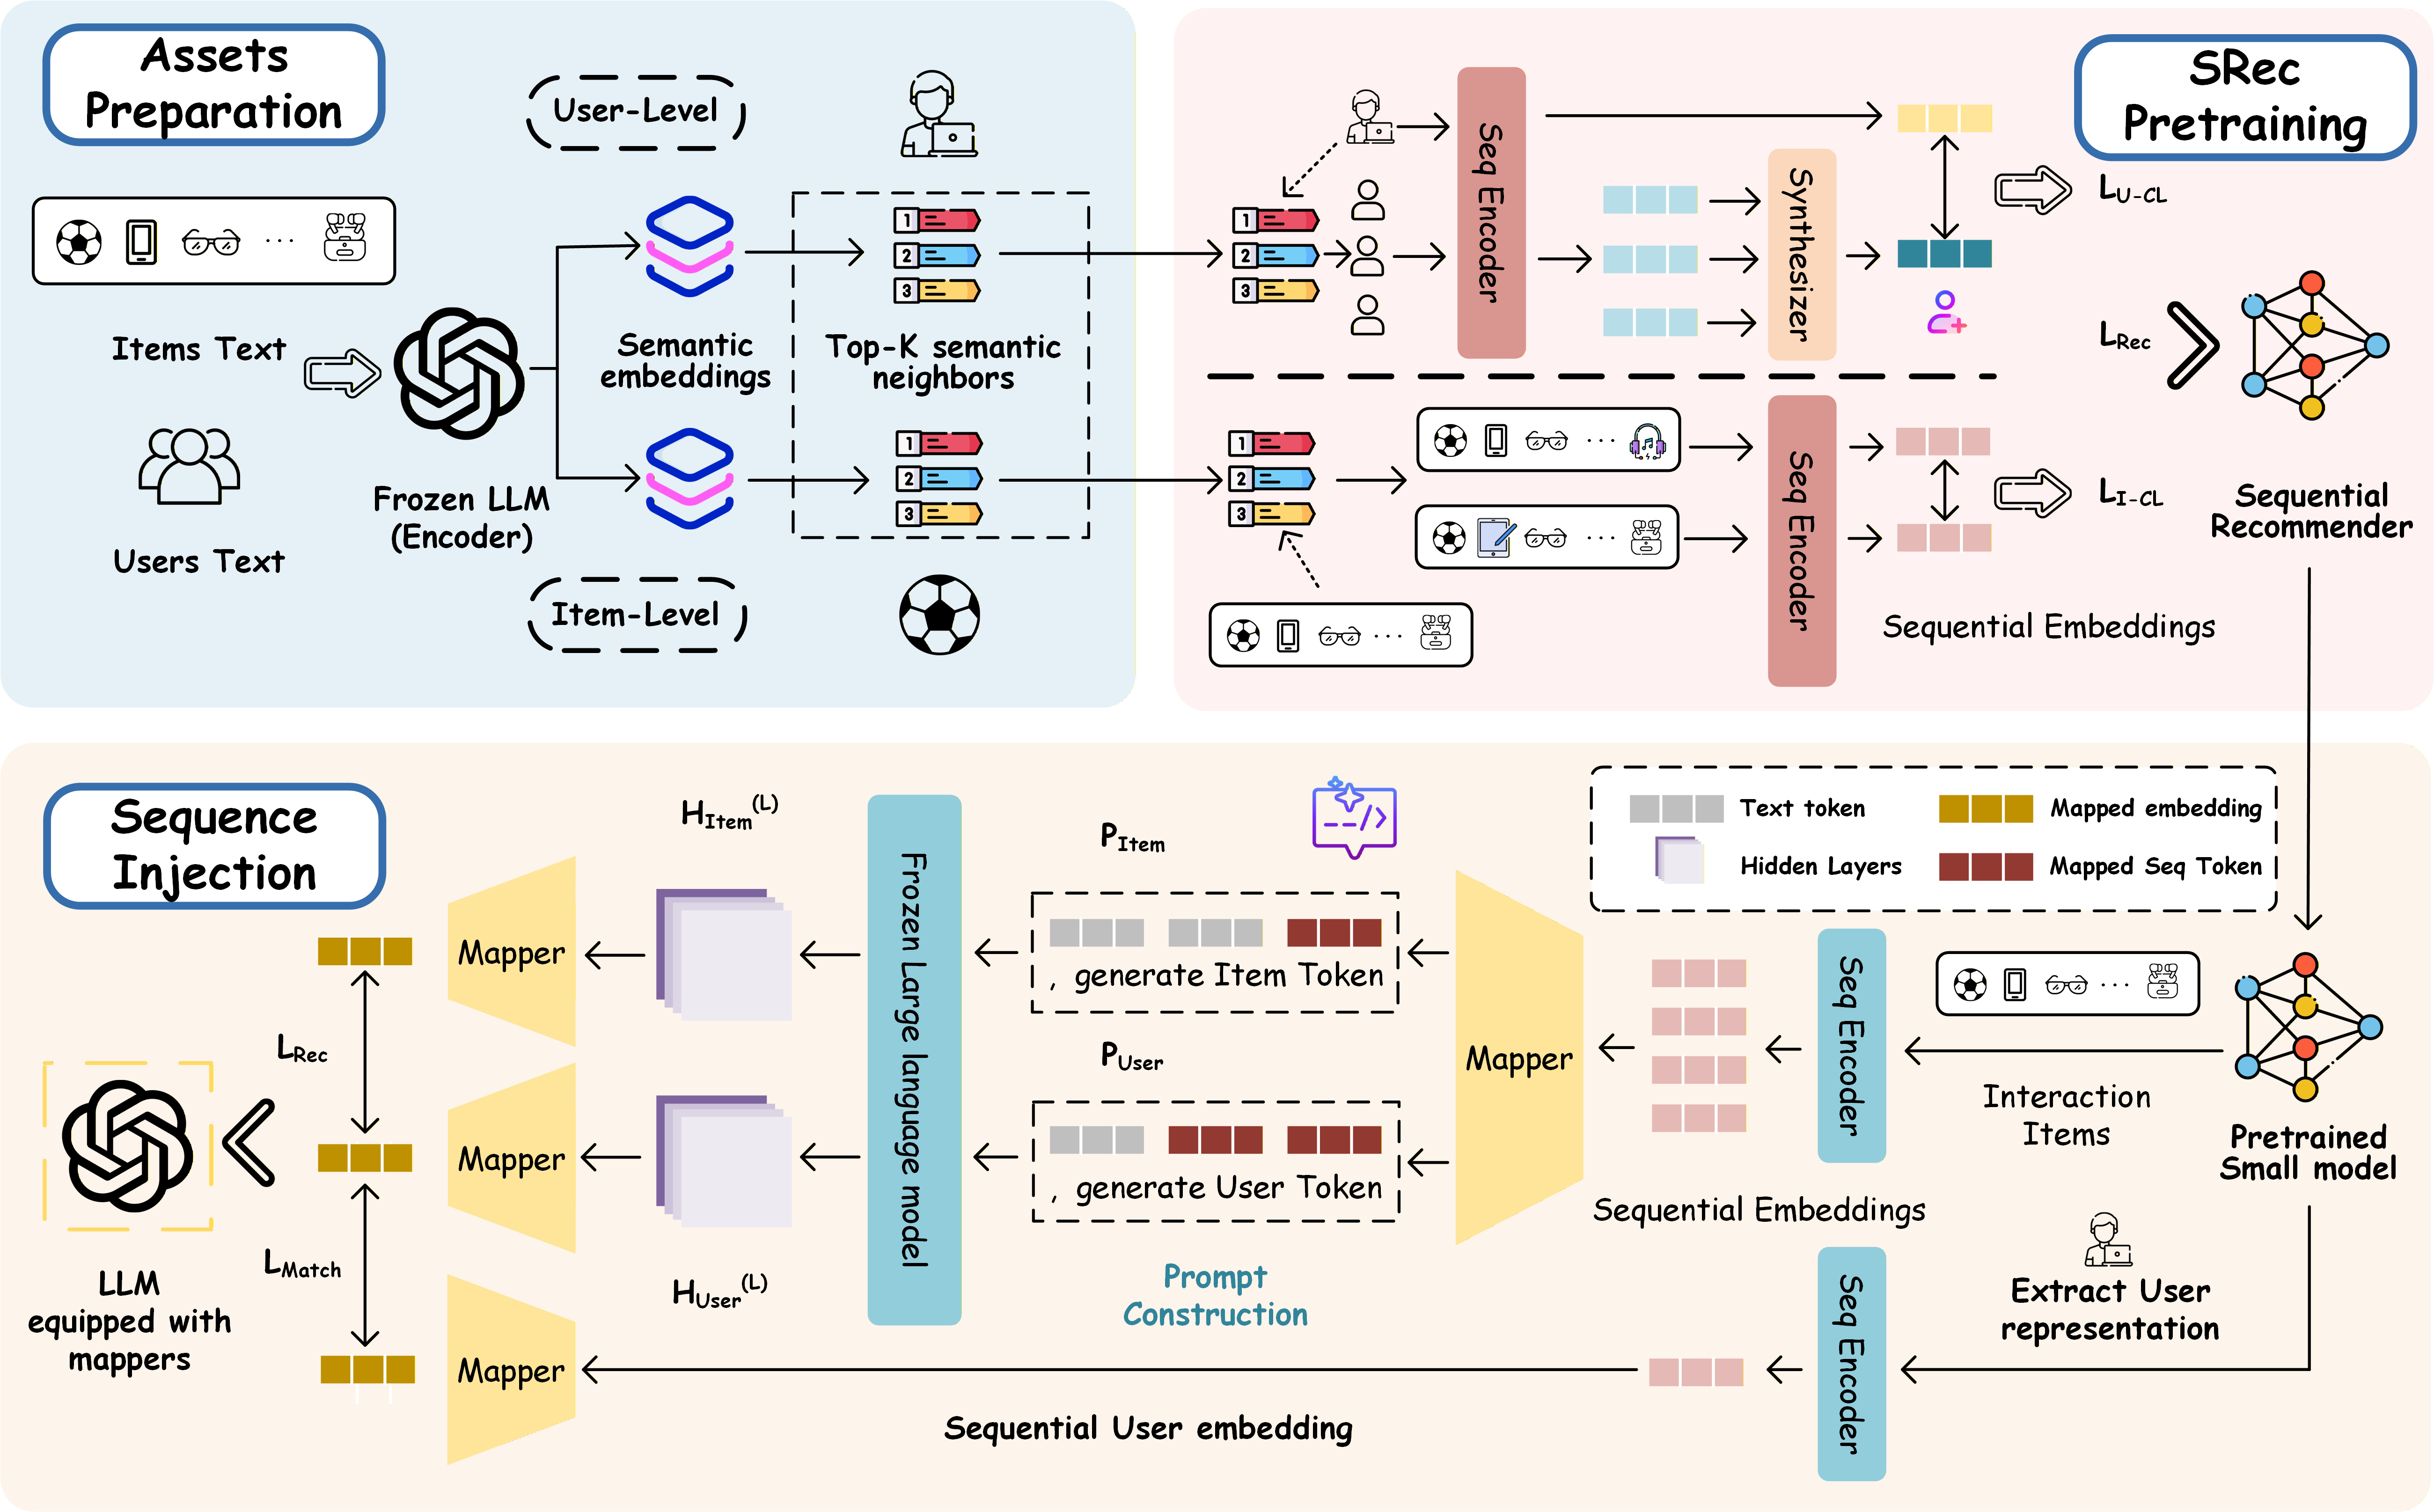
\includegraphics[draft=false,width=\textwidth]{EchoRec0415.png}%
\caption{Overall architecture of EchoRec. A frozen LLM first builds semantic assets for large-small collaboration. Stage I then reshapes the sequential teacher with SACP, and Stage II injects refined sequential embeddings into the frozen LLM via SI.}
\label{fig:echorec_architecture}
\end{figure*}

\subsection{Semantic Asset Preparation}

\noindent\textbf{Definition (Semantic assets).} \textit{Semantic assets are frozen LLM-derived item/user embeddings and semantic-neighborhood tables.}

To guide reshaping without leakage or LLM updates, we build these frozen anchors from item titles/metadata and training-prefix user histories, excluding validation and test target items. For an item or user-history text $x$, let the last-layer hidden output be $\mathbf{H}^{(L)}(x)\in\mathbb{R}^{L_x\times d_{sem}}$ with attention mask $\mathbf{m}\in\{0,1\}^{L_x}$. We obtain its semantic vector by masked mean pooling:
\begin{equation}
\mathrm{Enc}_{sem}(x)=
\mathrm{Norm}\!\left(
\frac{\sum_{t=1}^{L_x} m_t \mathbf{H}^{(L)}_t(x)}
{\sum_{t=1}^{L_x} m_t}
\right),
\end{equation}
where $\mathrm{Norm}(\cdot)$ denotes vector normalization. For nodes $v$ and $v'$, the semantic similarity is computed as follows:
\begin{equation}
s^{sem}(v,v')
=
\frac{(\mathbf{e}_v^{sem})^\top \mathbf{e}_{v'}^{sem}}
{\|\mathbf{e}_v^{sem}\|_2\|\mathbf{e}_{v'}^{sem}\|_2},
\end{equation}
where $\mathbf{e}_v^{sem}$ and $\mathbf{e}_{v'}^{sem}$ are frozen semantic vectors for nodes $v$ and $v'$, respectively. We then cache the corresponding semantic neighborhood:
\begin{equation}
\mathcal{N}_{sem}^{K}(v)
=
\operatorname*{Top\text{-}K}_{v'\in\mathcal{V}\setminus\{v\}}
\ s^{sem}(v,v'),
\end{equation}
where $\mathcal{V}$ is the node universe. These assets are never updated during training. Item neighborhoods provide semantic-preserving substitutions, and user-history neighborhoods provide local semantic regions that the teacher should not fragment.

\subsection{Stage I: Semantic-Aligned Contrastive Pre-training}

Although semantic assets provide references, the original teacher remains ID-dominated and may suffer from local semantic metric mismatch and semantic neighborhood fragmentation. SACP reshapes the sequential space before injection while preserving next-item supervision and adding complementary item-level and user-level semantic constraints for transfer readiness.

\noindent\textbf{Sequential teacher representation.} Let $\mathcal B$ be a mini-batch, $\mathbf{z}_u^{raw}\in\mathbb{R}^{d_s}$ the last-position output of $G_{sr}$ for $S_u$, and $\mathbf{r}_u$ its contrastive-head projection. Stage I first preserves the teacher's next-item discrimination~ability:
\begin{equation}
\mathcal{L}_{rec}^{sr}
=-\frac{1}{|\mathcal{B}|}\sum_{u\in\mathcal{B}}
\log
\frac{\exp\big((\mathbf{z}_u^{raw})^\top \mathbf{q}_{y_u}\big)}
{\sum_{j\in\mathcal I}\exp\big((\mathbf{z}_u^{raw})^\top \mathbf{q}_{j}\big)},
\end{equation}
where $\mathbf{q}_j$ is the item embedding.

\noindent\textbf{Item-level semantic replacement consistency.} Fully random item replacement can destroy the user's intent and create false positives. EchoRec instead builds two views $\tilde{S}_u^{(1)}$ and $\tilde{S}_u^{(2)}$ by replacing only a subset of items with neighbors from the frozen item semantic table. After re-encoding the views, we optimize:
\begin{equation}
\mathcal{L}_{i\text{-}cl}
=-\frac{1}{|\mathcal{B}|}\sum_{u\in\mathcal{B}}
\log
\frac{\exp(\mathrm{sim}(\mathbf{r}_u^{(1)},\mathbf{r}_u^{(2)})/\tau_s)}
{\sum_{v\in\mathcal{B}}
\exp(\mathrm{sim}(\mathbf{r}_u^{(1)},\mathbf{r}_v^{(2)})/\tau_s)},
\end{equation}
where $\mathbf{r}_u^{(1)}$ and $\mathbf{r}_u^{(2)}$ are projected views, $\mathrm{sim}(\cdot,\cdot)$ is cosine similarity, and $\tau_s$ is the temperature. This branch makes the teacher less tied to exact item IDs when the substituted items preserve semantics.

\noindent\textbf{User-level semantic aggregation.} Item-level consistency alone does not ensure that semantically similar histories occupy a coherent teacher region. For $\mathcal{N}_{u,\mathrm{sem}}^K:=\mathcal{N}_{sem}^{K}(u)$, EchoRec forms a soft semantic neighborhood target:
\begin{equation}
w_{u,v}
=
\frac{\exp(\kappa(\mathbf{e}_u^{sem},\mathbf{e}_v^{sem})/\tau_u)}
{\sum_{v'\in\mathcal{N}_{u,\mathrm{sem}}^K}\exp(\kappa(\mathbf{e}_u^{sem},\mathbf{e}_{v'}^{sem})/\tau_u)},
\end{equation}
where $w_{u,v}$ is the semantic neighborhood weight, $\kappa(\mathbf a,\mathbf b)=\mathbf a^\top\mathbf b/(\|\mathbf a\|_2\|\mathbf b\|_2)$, and $\tau_u>0$. The mixed neighborhood representation is:
\begin{equation}
\bar{\mathbf{r}}_u=\sum_{v\in\mathcal{N}_{u,\mathrm{sem}}^K}w_{u,v}\mathbf{r}_{v}^{seq},
\end{equation}
where $\mathbf{r}_{v}^{seq}$ encodes neighbor $v$'s training-prefix sequence. We use $\bar{\mathbf{r}}_u$ as the positive target:
\begin{equation}
\mathcal{L}_{u\text{-}cl}
=-\frac{1}{|\mathcal{B}|}\sum_{u\in\mathcal{B}}
\log
\frac{\exp(\mathrm{sim}(\mathbf{r}_u,\bar{\mathbf{r}}_u)/\tau_s)}
{\sum_{v\in\mathcal{B}}
\exp(\mathrm{sim}(\mathbf{r}_u,\bar{\mathbf{r}}_v)/\tau_s)},
\end{equation}
where $\bar{\mathbf{r}}_v$ is the mixed semantic neighborhood representation for user $v$. This branch reduces semantic neighborhood fragmentation in the teacher space.

\noindent\textbf{Objective function of Stage I.} Combining sequential recommendation supervision with the two semantic constraints, the Stage I objective is:
\begin{equation}
\mathcal{L}_{\text{SACP}}
=
\mathcal{L}_{rec}^{sr}
+\lambda_u \mathcal{L}_{u\text{-}cl}
+\lambda_i \mathcal{L}_{i\text{-}cl},
\end{equation}
where $\lambda_u$ and $\lambda_i$ control the two constraints. After optimization, the contrastive head is discarded; Stage II uses the reshaped backbone $G_{sr}^{+}$ and enhanced item table $E_{item}^{+}$.

\subsection{Stage II: Structure-aware Sequence Injection}

SACP makes the teacher more compatible with semantic references, but injection can still distort the reshaped structure. We therefore design SI to transfer the enhanced teacher into the frozen LLM without updating the LLM backbone. The goal is not to copy hidden states token by token, but to make the LLM-side retrieval representation preserve the teacher's discriminative user-item geometry.

\noindent\textbf{Teacher representation extraction and LLM reading.} Given $S_u$ and candidate set $\mathcal{C}_u$, the enhanced teacher outputs $\mathbf{z}_u^{+}=G_{sr}^{+}(S_u)$ and $\mathbf{c}_j=E_{item}^{+}(j)$. The projector $\Pi_{\phi}$ inserts each projected $\mathbf{c}_j$ at [ItemEmb] beside the item title. The frozen LLM produces [UserOut]/[ItemOut] states, and we set $\hat{\mathbf{u}}_u=f_u(\mathbf{h}_u^{\mathrm{UserOut}})$, $\hat{\mathbf{v}}_j=f_i(\mathbf{h}_j^{\mathrm{ItemOut}})$, and $\hat{\mathbf{t}}_u=M_{\psi}(\mathbf{z}_u^{+})$ in the retrieval subspace.

\noindent\textbf{Ranking loss and teacher matching loss.} Let $\mathcal{C}_u=\{j_u^{+},j_{u,1}^{-},\dots,j_{u,n-1}^{-}\}$ denote the candidate set. The user-item matching score in the shared retrieval subspace is:
\begin{equation}
s_{u,j}=\hat{\mathbf{u}}_u^{\top}\hat{\mathbf{v}}_j,
\label{eq:stage2_score}
\end{equation}
where $\hat{\mathbf{u}}_u$ and $\hat{\mathbf{v}}_j$ are LLM-side user and item representations.
Since the positive item is fixed at the first position during training, the Stage-II recommendation loss is:
\begin{equation}
\mathcal{L}_{rec}^{llm}
=-\frac{1}{|\mathcal{B}|}\sum_{u\in\mathcal{B}}
\log
\frac{\exp(s_{u,j_u^{+}})}
{\sum_{j\in\mathcal{C}_u}\exp(s_{u,j})},
\end{equation}
where $j_u^{+}$ is the positive item in $\mathcal{C}_u$.

Ranking alone can let the LLM-side user state drift toward generic semantic cues. We therefore match it to the enhanced teacher in the same retrieval subspace:
\begin{equation}
\mathcal{L}_{match}
=
\frac{1}{|\mathcal{B}|}\sum_{u\in\mathcal{B}}
\left\|
\overline{\mathbf{u}}_u-\overline{\mathbf{t}}_u
\right\|_2^2
+\mathcal{R}_{uni}(\overline{\mathbf U}_{\mathcal B})
+\mathcal{R}_{uni}(\overline{\mathbf T}_{\mathcal B}),
\label{eq:stage2_match}
\end{equation}
where $\overline{\mathbf U}_{\mathcal B}$ and $\overline{\mathbf T}_{\mathcal B}$ collect normalized $\hat{\mathbf u}_u$ and $\hat{\mathbf t}_u$ in the mini-batch, and $\mathcal{R}_{uni}(X)=\operatorname{mean}_{a<b}\exp(-2\|\mathbf{x}_a-\mathbf{x}_b\|_2^2)$. Thus, the ranking loss learns recommendation decisions, while the matching loss keeps injected user structure close to the reshaped teacher.

\noindent\textbf{Objective function of Stage II.} The objective is:
\begin{equation}
\mathcal{L}_{\text{SI}}=\mathcal{L}_{rec}^{llm}+\lambda_m\mathcal{L}_{match},
\end{equation}
where $\lambda_m$ controls teacher matching. Only $\Pi_{\phi}$, $f_u$, $f_i$, and $M_{\psi}$ are updated, with the LLM frozen.

\subsection{Retention View and Training Pipeline}
\label{sec:theory}

The pipeline above can be read as a sequence-retention mechanism. Appendix~\ref{app:theory} formalizes this view with local soft-neighborhood distributions, where the retained sequence signal is measured by how much the injected LLM-side neighborhood deviates from the reshaped teacher-side neighborhood. The resulting bound separates retention loss into three sources: teacher-space SSHG, a semantic-host residual, and injection-time drift.

This decomposition explains the training order. SACP targets the first term before transfer by using frozen semantic neighborhoods as local references, so the teacher no longer presents SI with a raw ID-dominated geometry. SI then controls the drift term by aligning the LLM-side user representation to the reshaped teacher while learning the ranking objective. The residual term records host-specific mismatch that is not directly optimized, which is why our diagnosis separately measures pre-injection alignment and post-injection structure transfer. Operationally, EchoRec follows three steps: build frozen semantic assets, reshape the teacher with $\mathcal{L}_{\text{SACP}}$, and inject the enhanced teacher with $\mathcal{L}_{\text{SI}}$.

\section{Experiments}
\label{sec:experiment}

We evaluate on four shared-benchmark datasets and ask:
\begin{itemize}[leftmargin=1.5em,itemsep=0pt,topsep=2pt]
\item \textbf{RQ1:} How does EchoRec compare with directly comparable baselines on the shared benchmark?
\item \textbf{RQ2:} Which components contribute most to the overall improvement?
\item \textbf{RQ3:} Is EchoRec robust under inference-time sequence perturbation?
\item \textbf{RQ4:} Does reducing SSHG improve alignment and structure transfer in controlled diagnosis?
\item \textbf{RQ5:} Is EchoRec effective across different sequential teacher backbones?
\end{itemize}

\subsection{Experimental setup}

\noindent\textbf{Datasets.} We follow the shared benchmark protocol of Kim et al.~\cite{kim2025lost} on four datasets: Movies, Scientific, Electronics, and CDs. For each user, we adopt the standard leave-one-out sequential split. Full dataset statistics are deferred to Appendix~\ref{app:datasets}.

\noindent\textbf{Evaluation Metrics.} Each test case is ranked against one positive item and 99 negative items. We report NDCG@10/20 and HR@10/20 for top-\(K\) ranking, and additionally report PreAlign@20, Jaccard@20, and RBO@20 for SSHG diagnosis; definitions are in Appendix~\ref{app:metrics}.

\noindent\textbf{Compared Methods.} Under the same retrieval-style protocol, we compare EchoRec with nine directly comparable baselines: GRU4Rec~\cite{hidasi2016gru4rec}, BERT4Rec~\cite{sun2019bert4rec}, NextItNet~\cite{yuan2019nextitnet}, SASRec~\cite{kang2018sasrec}, TALLRec~\cite{bao2023tallrec}, LLaRA~\cite{liao2024llara}, A-LLMRec~\cite{kim2024allmrec}, CoLLM~\cite{zhang2025collm}, and LLM-SRec~\cite{kim2025lost}. Detailed grouping and comparison notes are summarized in Appendix~\ref{app:baselines}.

\noindent\textbf{Implementation Details.} We follow the released protocols for directly comparable LLM4Rec baselines. EchoRec is model-agnostic and can be integrated with various sequential recommendation models. To introduce our approach, we adopt the Transformer architecture as the sequential teacher in the main setting, following prior studies on sequential recommendation~\cite{qin2023mclrec,cui2025sracl}. Section~\ref{subsec:model_agnostic} provides model-agnostic evaluation. Appendix~\ref{app:implementation} gives details.

\subsection{Overall performance on the shared benchmark (RQ1)}
\label{subsec:rq1}

Table~\ref{tab:main_overall} reports the unified benchmark comparison: the first four columns are conventional sequential recommenders, the next six are directly comparable LLM4Rec methods, and the rightmost column gives EchoRec's gain over the strongest prior LLM4Rec baseline. EchoRec achieves the best results on all datasets, with relative gains of 4.5\%--16.4\%. Conventional SRec models remain competitive but lack the LLM host's semantic reasoning, while prior LLM4Rec methods may still suffer when raw collaborative geometry conflicts with the LLM semantic space. EchoRec combines both sides: SACP reshapes the teacher space with frozen semantic neighborhoods, and SI injects a cleaner sequential signal. The gains hold on both NDCG and HR, indicating improvements in both top-rank ordering and candidate recall. The margin over LLM-SRec is meaningful because LLM-SRec already performs sequence-aware injection, suggesting that reshape-first reduces transfer difficulty before LLM-side alignment. The gains are especially visible on CDs and Movies, where sparse interactions and useful item text make direct ID-space transfer fragile. Sections~\ref{subsec:post-sacp} and~\ref{subsec:model_agnostic} further provide evidence that the gains are not merely from stronger injection and are not tied to one teacher backbone.

\begin{table*}[!t]
\centering
\caption{Overall performance on the shared benchmark of Kim et al.~\cite{kim2025lost}, with gains over the strongest prior LLM4Rec baseline in the rightmost column and best results in bold. EchoRec consistently improves ranking across datasets, showing the benefit of reshape-first sequence transfer.}
\label{tab:main_overall}
\small
\setlength{\tabcolsep}{2.8pt}
\renewcommand{\arraystretch}{1.06}
\resizebox{\textwidth}{!}{%
\begin{tabular}{c|c||c|c|c|c||c|c|c|c|c|c||c}
\toprule
\multirow{2}{*}{Dataset} & \multirow{2}{*}{Metric} & \multicolumn{4}{c||}{SRec} & \multicolumn{6}{c||}{LLM4Rec} & \multirow{2}{*}{\textbf{Improv.}} \\
\cmidrule(lr){3-6}\cmidrule(lr){7-12}
 &  & SASRec & GRU4Rec & BERT4Rec & NextItNet & TALLRec & LLaRA & A-LLMRec & CoLLM & LLM-SRec & EchoRec \\
\specialrule{0.4pt}{0.15ex}{0pt}
\specialrule{0.4pt}{0pt}{0.45ex}
\multirow{4}{*}{Movies}
 & NDCG@10 & 0.3459 & 0.3152 & 0.2959 & 0.2538 & 0.1668 & 0.1522 & 0.3263 & 0.3223 & 0.3560 & \textbf{0.4088} & +14.8\% \\
\cline{2-13}
 & NDCG@20 & 0.3745 & 0.3494 & 0.3303 & 0.2879 & 0.2126 & 0.1944 & 0.3629 & 0.3577 & 0.3924 & \textbf{0.4417} & +12.6\% \\
\cline{2-13}
 & HR@10 & 0.5180 & 0.4883 & 0.4785 & 0.4221 & 0.3234 & 0.2914 & 0.5127 & 0.5089 & 0.5569 & \textbf{0.6160} & +10.6\% \\
\cline{2-13}
 & HR@20 & 0.6310 & 0.6245 & 0.6213 & 0.5522 & 0.5060 & 0.4599 & 0.6577 & 0.6491 & 0.7010 & \textbf{0.7453} & +6.3\% \\
\specialrule{0.4pt}{0.35ex}{0pt}
\specialrule{0.4pt}{0pt}{0.45ex}
\multirow{4}{*}{Scientific}
 & NDCG@10 & 0.2918 & 0.2642 & 0.2576 & 0.2263 & 0.2585 & 0.2844 & 0.2875 & 0.3111 & 0.3388 & \textbf{0.3822} & +12.8\% \\
\cline{2-13}
 & NDCG@20 & 0.3245 & 0.2974 & 0.2913 & 0.2657 & 0.3048 & 0.3265 & 0.3246 & 0.3489 & 0.3758 & \textbf{0.4151} & +10.5\% \\
\cline{2-13}
 & HR@10 & 0.4691 & 0.4313 & 0.4437 & 0.3908 & 0.4574 & 0.4993 & 0.4957 & 0.5182 & 0.5532 & \textbf{0.6008} & +8.6\% \\
\cline{2-13}
 & HR@20 & 0.5987 & 0.5524 & 0.5822 & 0.5356 & 0.6276 & 0.6658 & 0.6427 & 0.6676 & 0.6992 & \textbf{0.7310} & +4.5\% \\
\specialrule{0.4pt}{0.35ex}{0pt}
\specialrule{0.4pt}{0pt}{0.45ex}
\multirow{4}{*}{Electronics}
 & NDCG@10 & 0.2267 & 0.2364 & 0.1867 & 0.1712 & 0.2249 & 0.2048 & 0.2791 & 0.2565 & 0.3044 & \textbf{0.3228} & +6.1\% \\
\cline{2-13}
 & NDCG@20 & 0.2606 & 0.2743 & 0.2172 & 0.2069 & 0.2670 & 0.2454 & 0.3173 & 0.2948 & 0.3424 & \textbf{0.3620} & +5.7\% \\
\cline{2-13}
 & HR@10 & 0.3749 & 0.3843 & 0.3325 & 0.3017 & 0.3802 & 0.3441 & 0.4622 & 0.4236 & 0.4885 & \textbf{0.5254} & +7.6\% \\
\cline{2-13}
 & HR@20 & 0.5096 & 0.5196 & 0.4740 & 0.4324 & 0.5476 & 0.5032 & 0.6137 & 0.5741 & 0.6385 & \textbf{0.6806} & +6.6\% \\
\specialrule{0.4pt}{0.35ex}{0pt}
\specialrule{0.4pt}{0pt}{0.45ex}
\multirow{4}{*}{CDs}
 & NDCG@10 & 0.3451 & 0.2155 & 0.3019 & 0.2207 & 0.3100 & 0.2464 & 0.3119 & 0.3152 & 0.3809 & \textbf{0.4432} & +16.4\% \\
\cline{2-13}
 & NDCG@20 & 0.3795 & 0.2530 & 0.3386 & 0.2562 & 0.3493 & 0.2951 & 0.3526 & 0.3557 & 0.4158 & \textbf{0.4761} & +14.5\% \\
\cline{2-13}
 & HR@10 & 0.5278 & 0.3712 & 0.5018 & 0.3842 & 0.5052 & 0.4665 & 0.5300 & 0.5290 & 0.6085 & \textbf{0.6796} & +11.7\% \\
\cline{2-13}
 & HR@20 & 0.6635 & 0.5092 & 0.6605 & 0.5422 & 0.6633 & 0.6590 & 0.6914 & 0.6895 & 0.7461 & \textbf{0.8094} & +8.5\% \\
\bottomrule
\end{tabular}}
\end{table*}

\subsection{Ablation study (RQ2)}

Table~\ref{tab:ablation_all} shows a stable hierarchy across datasets. Removing teacher-side reshaping (\textbf{w/o SACP}) causes the largest drops: NDCG@10 falls from 0.4088 to 0.3697 on Movies, 0.3822 to 0.3170 on Scientific, 0.3228 to 0.2756 on Electronics, and 0.4432 to 0.3733 on CDs. This suggests that the main gain is not simply from adding an LLM-side projector; when the teacher space remains noisy or fragmented, SI must both repair local structure and transfer across spaces. The single-component removals are smaller and complementary: Item-CL reduces sensitivity to exact ID substitutions, User-CL improves neighborhood coherence, and Match keeps the injected LLM user state near the reshaped sequential subspace. Overall, SACP prepares the teacher for reliable injection, while the consistent drops across domains support the staged design rather than a dataset-specific effect.

\begin{table}[!t]
\centering
\caption{Ablation results on all four datasets, where each row removes one EchoRec component and best results are in bold. The largest drops occur without SACP, indicating that teacher-side reshaping is the main source of improvement.}
\label{tab:ablation_all}
\small
\setlength{\tabcolsep}{2.8pt}
\renewcommand{\arraystretch}{1.06}
\resizebox{0.86\textwidth}{!}{%
\begin{tabular}{l||c|c||c|c||c|c||c|c}
\toprule
 \multicolumn{1}{c||}{\multirow{2}{*}{Method}} & \multicolumn{2}{c||}{Movies} & \multicolumn{2}{c||}{Scientific} & \multicolumn{2}{c||}{Electronics} & \multicolumn{2}{c}{CDs} \\
\cmidrule(lr){2-3}\cmidrule(lr){4-5}\cmidrule(lr){6-7}\cmidrule(lr){8-9}
 & NDCG@10 & HR@10 & NDCG@10 & HR@10 & NDCG@10 & HR@10 & NDCG@10 & HR@10 \\
\specialrule{0.4pt}{0.15ex}{0pt}
\specialrule{0.4pt}{0pt}{0.45ex}
EchoRec & \textbf{0.4088} & \textbf{0.6160} & \textbf{0.3822} & \textbf{0.6008} & \textbf{0.3228} & \textbf{0.5254} & \textbf{0.4432} & \textbf{0.6796} \\
\cline{1-9}
w/o User-CL & 0.3976 & 0.5988 & 0.3704 & 0.5816 & 0.3086 & 0.5030 & 0.4236 & 0.6586 \\
\cline{1-9}
w/o Item-CL & 0.4017 & 0.6036 & 0.3679 & 0.5814 & 0.3127 & 0.4998 & 0.4368 & 0.6674 \\
\cline{1-9}
w/o Match & 0.3986 & 0.6012 & 0.3753 & 0.5916 & 0.3174 & 0.5124 & 0.4266 & 0.6622 \\
\cline{1-9}
w/o SACP & 0.3697 & 0.5667 & 0.3170 & 0.5230 & 0.2756 & 0.4584 & 0.3733 & 0.5960 \\
\bottomrule
\end{tabular}
\vspace{0pt}}
\end{table}

\newpage
\subsection{Sequence perturbation stability (RQ3)}
\label{subsec:seq-perturb}

Figure~\ref{fig:seq_perturb_panel} evaluates inference-time sequence perturbations on CDs under original, shuffle, reverse, and recent-item removal settings. EchoRec keeps higher clean-input performance and degrades less under moderate perturbations such as shuffle and recent-item removal. Randomized perturbations are repeated with seeds 42, 52, and 62 and show the same trend. This suggests that EchoRec does not merely memorize item IDs or prompt surface forms; the SACP teacher learns smoother semantic neighborhoods, making small history changes less likely to cause abrupt drift after SI. Full reversal still hurts both methods, as desired, because chronological preference evolution is central to sequential recommendation. Thus, EchoRec better balances robustness and order sensitivity: it tolerates moderate noise while still responding to severe temporal disruption. Additional Movies, Scientific, and Electronics results are deferred to Appendix~\ref{app:seq_perturb_scientific}.
\begin{figure}[!t]
\centering
\begin{minipage}[t]{0.497\textwidth}
\vspace{0pt}
\centering
\begin{minipage}[t]{0.495\linewidth}
\centering
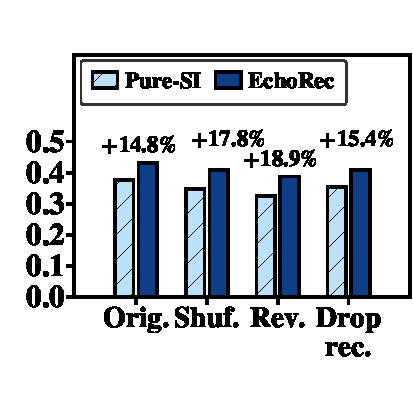
\includegraphics[width=\linewidth,trim=0 22pt 0 0,clip]{sequence_perturb_cds_ndcg10_crop.pdf}
\vspace{-0.60em}
\axissubcaption{(a) NDCG@10}
\end{minipage}\hfill
\begin{minipage}[t]{0.495\linewidth}
\centering
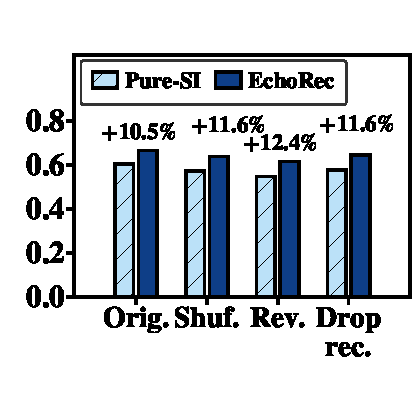
\includegraphics[width=\linewidth,trim=0 22pt 0 0,clip]{sequence_perturb_cds_hr10_crop.pdf}
\vspace{-0.60em}
\axissubcaption{(b) HR@10}
\end{minipage}
\captionsetup{type=figure,skip=2pt,justification=raggedright,singlelinecheck=false,margin=0pt}
\captionof{figure}{Sequence perturbation under input-history perturbations.}
\label{fig:seq_perturb_panel}
\end{minipage}\hfill
\begin{minipage}[t]{0.497\textwidth}
\vspace{0pt}
\centering
\begin{minipage}[t]{0.495\linewidth}
\centering

\includegraphics[width=\linewidth,trim=0 22pt 0 0,clip]{cds_sshg_semantic.pdf}
\vspace{-0.60em}
\axissubcaption{(a) Semantic Alignment}
\end{minipage}\hfill
\begin{minipage}[t]{0.495\linewidth}
\centering

\includegraphics[width=\linewidth,trim=0 22pt 0 0,clip]{cds_sshg_transfer.pdf}
\vspace{-0.60em}
\axissubcaption{(b) Structure Transfer}
\end{minipage}
\captionsetup{type=figure,skip=2pt,justification=raggedright,singlelinecheck=false,margin=0pt}
\captionof{figure}{Controlled SSHG diagnosis across neighborhood scales.}
\label{fig:cds_scientific_sshg_curves}
\end{minipage}
\vspace{-0.6em}
\end{figure}

\subsection{Controlled SSHG diagnosis (RQ4)}
\label{subsec:post-sacp}

With the dataset, LLM backbone, protocol, and budget fixed, Figure~\ref{fig:cds_scientific_sshg_curves} isolates teacher-space reshaping on CDs by comparing EchoRec with Pure-SI. EchoRec raises pre-injection semantic neighborhood overlap in panel (a) and post-injection structure transfer in panel (b), showing that SACP reduces the projector's burden: SI receives a teacher space whose local neighborhoods are already more compatible with frozen semantic neighborhoods, preserving teacher-side overlap and rank fidelity in the LLM space rather than repairing raw ID-space geometry.

Table~\ref{tab:multidataset_sshg_delta} extends this diagnosis to all datasets under the same neighborhood scale. EchoRec consistently improves pre-injection semantic alignment, post-injection neighborhood overlap, rank fidelity, and downstream NDCG over Pure-SI. These gains provide proxy evidence that SACP prepares a teacher space more compatible with the frozen semantic host, allowing SI to transfer sequential structure with less distortion. Thus, reducing SSHG-related mismatch before injection is associated with better structure preservation and recommendation quality, with correlations in Appendix~\ref{app:diagnosis_relation}.

\begin{table}[!t]
\centering
\caption{Cross-dataset SSHG diagnosis at $k=20$ on 2,000 sampled prefixes per seed, reporting Pure-SI, EchoRec, and relative gains. The rows trace a diagnostic progression from pre-injection semantic alignment to post-injection structure transfer and downstream ranking quality.}
\label{tab:multidataset_sshg_delta}
\small
\setlength{\tabcolsep}{2.8pt}
\renewcommand{\arraystretch}{1.06}
\resizebox{\textwidth}{!}{%
\begin{tabular}{l||c|c|c||c|c|c||c|c|c||c|c|c}
\toprule
\multicolumn{1}{c||}{\multirow{2}{*}{Metric}}
& \multicolumn{3}{c||}{Movies}
& \multicolumn{3}{c||}{Scientific}
& \multicolumn{3}{c||}{Electronics}
& \multicolumn{3}{c}{CDs} \\
\cmidrule(lr){2-4}\cmidrule(lr){5-7}\cmidrule(lr){8-10}\cmidrule(lr){11-13}
& Pure-SI & EchoRec & \textbf{Improv.}
& Pure-SI & EchoRec & \textbf{Improv.}
& Pure-SI & EchoRec & \textbf{Improv.}
& Pure-SI & EchoRec & \textbf{Improv.} \\
\specialrule{0.4pt}{0.15ex}{0pt}
\specialrule{0.4pt}{0pt}{0.45ex}
PreAlign@20
& 0.0245 & 0.0471 & \textbf{+92.4\%}
& 0.0276 & 0.0654 & \textbf{+136.7\%}
& 0.0166 & 0.0500 & \textbf{+200.4\%}
& 0.0331 & 0.0535 & \textbf{+61.6\%} \\
\cline{1-13}
Jaccard@20
& 0.0529 & 0.1053 & \textbf{+99.0\%}
& 0.0790 & 0.1625 & \textbf{+105.6\%}
& 0.0415 & 0.0850 & \textbf{+104.8\%}
& 0.1155 & 0.1934 & \textbf{+67.5\%} \\
\cline{1-13}
RBO@20
& 0.0544 & 0.1234 & \textbf{+126.9\%}
& 0.0995 & 0.1885 & \textbf{+89.4\%}
& 0.0541 & 0.1036 & \textbf{+91.3\%}
& 0.1297 & 0.2283 & \textbf{+75.9\%} \\
\cline{1-13}
NDCG@10
& 0.3657 & 0.4088 & \textbf{+11.8\%}
& 0.3137 & 0.3797 & \textbf{+21.0\%}
& 0.2736 & 0.3313 & \textbf{+21.1\%}
& 0.3718 & 0.4275 & \textbf{+15.0\%} \\
\bottomrule
\end{tabular}
\vspace{0pt}}
\end{table}

\subsection{Model-agnostic evaluation (RQ5)}
\label{subsec:model_agnostic}

We further test whether EchoRec is model-agnostic by integrating the full pipeline with GRU4Rec, SASRec, and BERT4Rec teacher backbones under the same LLM host and protocol. Figure~\ref{fig:model_agnostic_main} shows consistent improvements on both CDs and Movies across all three teachers. The gains across recurrent, self-attentive, and bidirectional encoders indicate that EchoRec is an extensible framework whose teacher-space reshaping mechanism is not tied to a specific sequential backbone.

\begin{figure}[!t]
\centering
\begin{minipage}[t]{0.2485\textwidth}
\centering
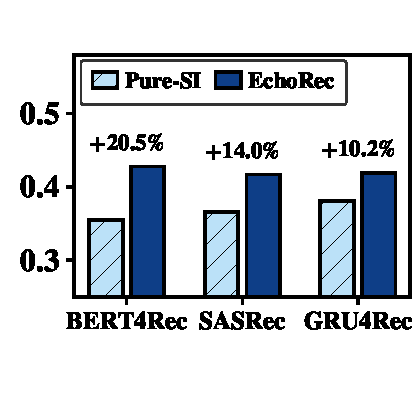
\includegraphics[width=\linewidth,trim=0 36pt 0 0,clip]{model_agnostic_cds_ndcg10.pdf}
\vspace{-0.60em}
\axissubcaption{(a) CDs NDCG@10}
\end{minipage}\hfill
\begin{minipage}[t]{0.2485\textwidth}
\centering
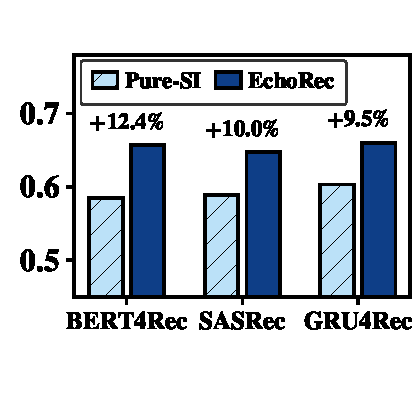
\includegraphics[width=\linewidth,trim=0 36pt 0 0,clip]{model_agnostic_cds_hr10.pdf}
\vspace{-0.60em}
\axissubcaption{(b) CDs HR@10}
\end{minipage}\hfill
\begin{minipage}[t]{0.2485\textwidth}
\centering
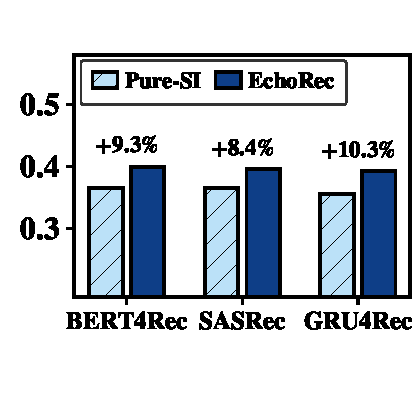
\includegraphics[width=\linewidth,trim=0 36pt 0 0,clip]{model_agnostic_movies_ndcg10.pdf}
\vspace{-0.60em}
\axissubcaption{(c) Movies NDCG@10}
\end{minipage}\hfill
\begin{minipage}[t]{0.2485\textwidth}
\centering
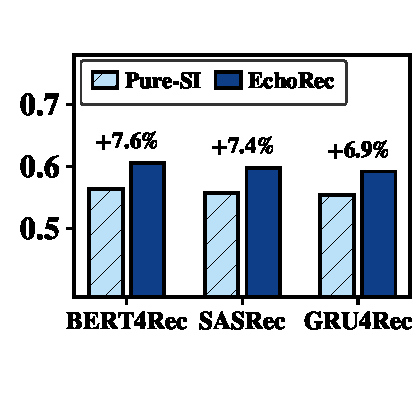
\includegraphics[width=\linewidth,trim=0 36pt 0 0,clip]{model_agnostic_movies_hr10.pdf}
\vspace{-0.60em}
\axissubcaption{(d) Movies HR@10}
\end{minipage}
\captionsetup{skip=2pt}
\caption{Model-agnostic evaluation with BERT4Rec, SASRec, and GRU4Rec teachers.}
\label{fig:model_agnostic_main}
\vspace{-0.6em}
\end{figure}

\section{Related Work}
\label{sec:related}

\noindent\textbf{Sequential Recommendation.} Sequential recommendation mainly focuses on identifying similar items or users from collaborative filtering signals and modeling how user preference evolves over interaction histories. Early methods combined matrix factorization with Markov transitions to capture temporal dynamics, such as FPMC~\cite{rendle2010fpmc}. Neural models then pushed this line forward: GRU4Rec~\cite{hidasi2016gru4rec} used recurrent architectures, NextItNet~\cite{yuan2019nextitnet} introduced convolutional sequence modeling, and later SASRec~\cite{kang2018sasrec} and BERT4Rec~\cite{sun2019bert4rec} further improved sequence representation with attention-based architectures. Recent studies such as ICLRec~\cite{chen2022iclrec}, C2lRec~\cite{xu2025c2lrec}, CMCLRec~\cite{xu2024cmclrec}, CLLMRec~\cite{lu2025cllmrec}, HPSERec~\cite{xu2025hpserec}, and FMLP-Rec~\cite{zhou2022fmlprec} continue to strengthen sequence learning through intent contrast, causal contrast, multimodal enhancement, LLM-based view augmentation, long-tail modeling, and lightweight encoders. These methods improve sequential discrimination but usually optimize within the collaborative space itself. Despite these advances, sequential recommender spaces are still mainly shaped by ID co-occurrence and exposure statistics, often lacking smooth and compatible semantic structure for transfer into an LLM host.

\noindent\textbf{LLM-based Recommendation.} With the rise of large language models, recommendation research has explored tighter ways of coupling LLMs with sequential signals~\cite{lin2025survey,zhao2024era}. Initial LLM-based recommenders mainly used LLMs as textual reasoning modules through prompting or lightweight tuning: TALLRec~\cite{bao2023tallrec} uses PEFT to bridge language modeling and recommendation, while ThinkRec~\cite{yu2026thinkrec} further introduces explicit reasoning. Since such text-only adaptation weakly captures collaborative patterns and sequential transitions, later work brought collaborative knowledge back into the LLM pipeline. LLaRA~\cite{liao2024llara} combines CF-SRec item embeddings with textual prompts, CoLLM~\cite{zhang2025collm} directly injects collaborative embeddings into the online LLM context, and A-LLMRec~\cite{kim2024allmrec} further strengthens CF knowledge absorption through representation alignment. Recent work further exposes weak dynamic-preference modeling in LLM4Rec and introduces sequence-aware distillation~\cite{kim2025lost}. A parallel direction uses LLMs to enhance smaller recommenders, including RLMRec~\cite{ren2024rlmrec}, LLM-ESR~\cite{liu2024llmesr}, SRA-CL~\cite{cui2025sracl}, LLMEmb~\cite{liu2025llmemb}, and large-small collaboration methods~\cite{zhang2026crossscale,lv2025lsc4rec}, while related efforts explore collaborative retrieval augmentation~\cite{wu2024coral}, plug-in LLM contrastive representations~\cite{wang2025piccdr}, logical or role-aware recommendation~\cite{yu2025tagcf}, and token-level collaborative alignment~\cite{lin2026tca4rec}.

Inspired by recent large-small collaboration studies, we argue that these two directions should be treated as a staged compatibility problem rather than separate pipelines. Existing methods mainly focus on injection-time alignment or distillation, largely overlooking structural mismatch between the teacher space and the LLM host. EchoRec instead uses frozen LLM semantics to reshape the small teacher before transfer, motivating preparation before injection for lower-distortion sequence transfer and more stable LLM-side sequential utilization under moderate perturbations.
 
\section{Conclusion}
We study SSHG in LLM-enhanced sequential recommendation and propose EchoRec, a staged large-small model collaboration framework. EchoRec builds frozen semantic assets, reshapes the sequential teacher with SACP, and injects the refined teacher space into the frozen LLM through SI. Experiments, ablations, perturbation analysis, SSHG diagnosis, and backbone generality studies show consistent gains and provide evidence that preparing a compatible teacher space improves sequence transfer before injection. Overall, EchoRec supports a reshape-first, inject-later strategy for lower-distortion LLM-based sequential recommendation.

\begin{thebibliography}{99}
\bibitem{xu2025hpserec}
Xiaolong Xu, Xudong Zhao, Haolong Xiang, Xuyun Zhang, Wei Shen, Hongsheng Hu, and Lianyong Qi. 2025.
HPSERec: A Hierarchical Partitioning and Stepwise Enhancement Framework for Long-tailed Sequential Recommendation.
In \textit{Advances in Neural Information Processing Systems 39 (NeurIPS '25)}.

\bibitem{liu2025recbench}
Qijiong Liu, Jieming Zhu, Lu Fan, Kun Wang, Hengchang Hu, Wei Guo, Yong Liu, and Xiao-Ming Wu. 2025.
Can LLMs Outshine Conventional Recommenders? A Comparative Evaluation.
In \textit{Advances in Neural Information Processing Systems 39 (NeurIPS '25)}.

\bibitem{lin2026tca4rec}
Zhuowei Lin, Huan Yao, Xingchen Ma, Ruiran Yan, Yuxiang Ren, Xian Wu, Zhixiang Zhang, and Yong Li. 2026.
Token-level collaborative alignment for LLM-based generative recommendation.
In \textit{Proceedings of the ACM Web Conference 2026 (WWW '26)}. ACM.

\bibitem{yu2025tagcf}
Qing Yu, Xiaobei Wang, Shuchang Liu, Yandong Bai, Xiaoyu Yang, Xueliang Wang, Chang Meng, Shanshan Wu, Hailan Yang, Bin Wen, Huihui Xiao, Xiang Li, Fan Yang, Xiaoqiang Feng, Lantao Hu, Han Li, Kun Gai, and Lixin Zou. 2025.
Who You Are Matters: Bridging Topics and Social Roles via LLM-Enhanced Logical Recommendation.
In \textit{Advances in Neural Information Processing Systems 39 (NeurIPS '25)}.

\bibitem{lv2025lsc4rec}
Zheqi Lv, Hongyan Zhao, Han Wang, Yang Song, Yongsheng Zhang, Yuxiang Wang, and Dawei Yin. 2025.
Collaboration of large language models and small recommendation models for device-cloud recommendation.
In \textit{Proceedings of the 31st ACM SIGKDD Conference on Knowledge Discovery and Data Mining (KDD '25)}. ACM.

\bibitem{xu2024cmclrec}
Xiaolong Xu, Hongsheng Dong, Lianyong Qi, Xuyun Zhang, Haolong Xiang, Xiaoyu Xia, Yanwei Xu, and Wanchun Dou. 2024.
CMCLRec: Cross-modal Contrastive Learning for User Cold-start Sequential Recommendation.
In \textit{Proceedings of the 47th International ACM SIGIR Conference on Research and Development in Information Retrieval (SIGIR '24)}. ACM, 1589--1598.

\bibitem{you2025r2ec}
Runyang You, Yongqi Li, Xinyu Lin, Xin Zhang, Wenjie Wang, Wenjie Li, and Liqiang Nie. 2025.
R2ec: Towards Large Recommender Models with Reasoning.
In \textit{Advances in Neural Information Processing Systems 39 (NeurIPS '25)}.

\bibitem{lu2025cllmrec}
Fan Lu, Xiaolong Xu, Haolong Xiang, Lianyong Qi, Xiaokang Zhou, Fei Dai, and Wanchun Dou. 2025.
CLLMRec: Contrastive Learning with LLMs-based View Augmentation for Sequential Recommendation.
In \textit{Proceedings of the Thirty-Fourth International Joint Conference on Artificial Intelligence (IJCAI '25)}. 3153--3161.

\bibitem{wang2026contextbias}
Yue Wang, Guibiao Wang, Mingde Yao, Jiawei Chen, Xin Xin, and Fuli Feng. 2026.
Does LLM focus on the right words? Mitigating context bias in LLM-based recommenders.
In \textit{Proceedings of the ACM Web Conference 2026 (WWW '26)}. ACM.

\vspace{-0.45em}

\bibitem{xu2025c2lrec}
Xiaolong Xu, Hongsheng Dong, Haolong Xiang, Xiyuan Hu, Xiaoyong Li, Xiaoyu Xia, Xuyun Zhang, Lianyong Qi, and Wanchun Dou. 2025.
C2lRec: Causal Contrastive Learning for User Cold-start Recommendation with Social Variables.
\textit{ACM Transactions on Information Systems} 43, 6 (2025), 143:1--143:28.

\bibitem{yu2026thinkrec}
Qihang Yu, Kairui Fu, Zheqi Lv, Shengyu Zhang, Xinhui Wu, Chen Lin, Feng Wei, Bo Zheng, and Wenwu Ou. 2026.
ThinkRec: Thinking-based recommendation via LLM.
In \textit{Proceedings of the ACM Web Conference 2026 (WWW '26)}. ACM.

\bibitem{zhang2026crossscale}
Yipeng Zhang, Xin Wang, Hong Chen, Junwei Pan, Qian Li, Jun Zhang, Jie Jiang, Hong Mei, and Wenwu Zhu. 2026.
Cross-Scale Collaboration between LLMs and Lightweight Sequential Recommenders with Domain-Specific Latent Reasoning.
In \textit{Proceedings of the AAAI Conference on Artificial Intelligence (AAAI '26)}.

\bibitem{he2025llm2rec}
Yingzhi He, Xiaohao Liu, An Zhang, Yunshan Ma, and Tat-Seng Chua. 2025.
LLM2Rec: Large language models are powerful embedding models for sequential recommendation.
In \textit{Proceedings of the 31st ACM SIGKDD Conference on Knowledge Discovery and Data Mining (KDD '25)}. ACM.

\bibitem{hong2025eagerllm}
Minjie Hong, Yan Xia, Zehan Wang, Jieming Zhu, Ye Wang, and Sihang Cai. 2025.
EAGER-LLM: Enhancing large language models as recommenders through exogenous behavior-semantic integration.
In \textit{Proceedings of the ACM Web Conference 2025 (WWW '25)}. ACM.

\bibitem{cui2025sracl}
Ziqiang Cui, Yunpeng Weng, Xing Tang, Xiaokun Zhang, Shiwei Li, Peiyang Liu, Bowei He, Dugang Liu, Weihong Luo, Xiuqiang He, and Chen Ma. 2025.
SRA-CL: Semantic retrieval augmented contrastive learning for sequential recommendation.
In \textit{Advances in Neural Information Processing Systems 39 (NeurIPS '25)}.

\bibitem{liu2025llmemb}
Qidong Liu, Xian Wu, Wanyu Wang, Yejing Wang, Yuanshao Zhu, Xiangyu Zhao, Feng Tian, and Yefeng Zheng. 2025.
LLMEmb: Large language model can be a good embedding generator for sequential recommendation.
In \textit{Proceedings of the AAAI Conference on Artificial Intelligence (AAAI '25)}.

\bibitem{kim2025lost}
Kibum Kim, Hongseok Kang, Sein Kim, Jiwan Kim, Donghyun Kim, Minchul Yang, and Chanyoung Park. 2025.
Lost in sequence: Do large language models understand sequential recommendation?
In \textit{Proceedings of the 31st ACM SIGKDD Conference on Knowledge Discovery and Data Mining (KDD '25)}. ACM.

\bibitem{wang2025piccdr}
Ke Wang, Ji Zhang, and Kuan Liu. 2025.
Enhancing cross-domain recommendation with plug-in contrastive representations from large language models.
In \textit{Proceedings of the 48th International ACM SIGIR Conference on Research and Development in Information Retrieval (SIGIR '25)}. ACM.

\bibitem{wang2025pad}
Yuhao Wang, Junwei Pan, Pengyue Jia, Wanyu Wang, Maolin Wang, Zhixiang Feng, Xiaotian Li, Jie Jiang, and Xiangyu Zhao. 2025.
Pre-train, align, and disentangle: Empowering sequential recommendation with large language models.
In \textit{Proceedings of the 48th International ACM SIGIR Conference on Research and Development in Information Retrieval (SIGIR '25)}. ACM.

\bibitem{liao2024llara}
Zhiyu Liao, Xujiang Zhao, Le Wu, Jingjing Li, Xing Xie, and Peng Cui. 2024.
LLaRA: Large language-recommendation assistant.
In \textit{Proceedings of the 47th International ACM SIGIR Conference on Research and Development in Information Retrieval (SIGIR '24)}. ACM.

\bibitem{kim2024allmrec}
Sein Kim, Hongseok Kang, Seungyoon Choi, Donghyun Kim, Minchul Yang, and Chanyoung Park. 2024.
Large language models meet collaborative filtering: An efficient all-round LLM-based recommender system.
In \textit{Proceedings of the 30th ACM SIGKDD Conference on Knowledge Discovery and Data Mining (KDD '24)}. ACM.

\bibitem{wu2024coral}
Junda Wu, Cheng-Chun Chang, Tong Yu, Zhankui He, Jianing Wang, Yupeng Hou, and Julian McAuley. 2024.
Coral: Collaborative retrieval-augmented large language models improve long-tail recommendation.
In \textit{Proceedings of the 30th ACM SIGKDD Conference on Knowledge Discovery and Data Mining (KDD '24)}. ACM, 3391--3401.

\bibitem{ren2024rlmrec}
Xubin Ren, Wei Wei, Lianghao Xia, Lixin Su, Suqi Cheng, Junfeng Wang, Dawei Yin, and Chao Huang. 2024.
Representation learning with large language models for recommendation.
In \textit{Proceedings of the ACM Web Conference 2024 (WWW '24)}. ACM, 3461--3472.

\bibitem{zheng2024trsr}
Zhi Zheng, Wenshuo Chao, Zhaopeng Qiu, Hengshu Zhu, and Hui Xiong. 2024.
Harnessing large language models for text-rich sequential recommendation.
In \textit{Proceedings of the ACM Web Conference 2024 (WWW '24)}. ACM, 3207--3216.

\bibitem{liu2024llmesr}
Qidong Liu, Xian Wu, Yejing Wang, Zijian Zhang, Feng Tian, Yefeng Zheng, and Xiangyu Zhao. 2024.
LLM-ESR: Large language models enhancement for long-tailed sequential recommendation.
In \textit{Advances in Neural Information Processing Systems 38 (NeurIPS '24)}.

\bibitem{qin2023mclrec}
Xiuyuan Qin, Huanhuan Yuan, Pengpeng Zhao, Junhua Fang, Fuzhen Zhuang, Guanfeng Liu, Yanchi Liu, and Victor S. Sheng. 2023.
Meta-optimized Contrastive Learning for Sequential Recommendation.
In \textit{Proceedings of the 46th International ACM SIGIR Conference on Research and Development in Information Retrieval (SIGIR '23)}. ACM, 89--98.

\bibitem{zhou2022fmlprec}
Kun Zhou, Hui Wang, Wayne Xin Zhao, and Ji-Rong Wen. 2022.
Filter-enhanced MLP is all you need for sequential recommendation.
In \textit{Proceedings of the ACM Web Conference 2022 (WWW '22)}. ACM, 2388--2399.

\bibitem{chen2022iclrec}
Yongjun Chen, Zhiwei Liu, Jia Li, Julian McAuley, and Caiming Xiong. 2022.
Intent contrastive learning for sequential recommendation.
In \textit{Proceedings of the ACM Web Conference 2022 (WWW '22)}. ACM, 2172--2182.

\bibitem{rendle2010fpmc}
Steffen Rendle, Christoph Freudenthaler, and Lars Schmidt-Thieme. 2010.
Factorizing personalized Markov chains for next-basket recommendation.
In \textit{Proceedings of the 19th International Conference on World Wide Web (WWW '10)}. ACM, 811--820.

\bibitem{wang2020alignment}
Tongzhou Wang and Phillip Isola. 2020.
Understanding contrastive representation learning through alignment and uniformity on the hypersphere.
In \textit{Proceedings of the 37th International Conference on Machine Learning (ICML '20)}. PMLR, 9929--9939.

\bibitem{hidasi2016gru4rec}
Bal\'azs Hidasi, Alexandros Karatzoglou, Linas Baltrunas, and Domonkos Tikk. 2016.
Session-based recommendations with recurrent neural networks.
In \textit{Proceedings of the 4th International Conference on Learning Representations (ICLR '16)}.

\bibitem{lin2025survey}
Jianghao Lin, Xinyi Dai, Yunjia Xi, Weiwen Liu, Bo Chen, Hao Zhang, Yong Liu, Chuhan Wu, Xiangyang Li, Chenxu Zhu, Huifeng Guo, Yong Yu, Ruiming Tang, and Weinan Zhang. 2025.
How can recommender systems benefit from large language models: A survey.
\textit{ACM Transactions on Information Systems} 43, 2 (2025), Article 28.

\bibitem{zhang2025collm}
Shuai Zhang, Keqin Bao, Yang Zhang, Yunxin Hu, Fuli Feng, Xiangnan He, and Xiang Wang. 2025.
CoLLM: Integrating collaborative embeddings into large language models for recommendation.
\textit{IEEE Transactions on Knowledge and Data Engineering} 37, 2 (2025), 1037--1051.

\bibitem{sun2019bert4rec}
Fei Sun, Jun Liu, Jian Wu, Changhua Pei, Xiao Lin, Wenwu Ou, and Peng Jiang. 2019.
BERT4Rec: Sequential recommendation with bidirectional encoder representations from transformer.
In \textit{Proceedings of the 28th ACM International Conference on Information and Knowledge Management (CIKM '19)}. ACM.

\bibitem{kang2018sasrec}
Wang-Cheng Kang and Julian McAuley. 2018.
Self-attentive sequential recommendation.
In \textit{Proceedings of the 18th IEEE International Conference on Data Mining (ICDM '18)}. IEEE.

\bibitem{yuan2019nextitnet}
Fajie Yuan, Xiangnan He, Alexandros Karatzoglou, and Lizi Zhang. 2019.
A simple convolutional generative network for next item recommendation.
In \textit{Proceedings of the Twelfth ACM International Conference on Web Search and Data Mining (WSDM '19)}. ACM.

\bibitem{bao2023tallrec}
Keqin Bao, Jizhi Zhang, Yang Zhang, Wenjie Wang, Fuli Feng, and Xiangnan He. 2023.
TALLRec: An effective and efficient tuning framework to align large language model with recommendation.
In \textit{Proceedings of the 17th ACM Conference on Recommender Systems (RecSys '23)}. ACM.

\bibitem{cover2006elements}
Thomas M. Cover and Joy A. Thomas. 2006.
\textit{Elements of Information Theory}, 2nd edition.
Wiley.

\bibitem{csiszar1967information}
Imre Csisz\'ar. 1967.
Information-type measures of difference of probability distributions and indirect observations.
\textit{Studia Scientiarum Mathematicarum Hungarica} 2 (1967), 299--318.

\bibitem{zhao2024era}
Zhe Zhao, Wei Fan, Junhao Li, Yuyang Liu, Xing Mei, Yongfeng Wang, Zhiqi Wen, Feng Wang, Xiangyu Zhao, Ji-Rong Wen, et al. 2024.
Recommender systems in the era of large language models (LLMs).
\textit{IEEE Transactions on Knowledge and Data Engineering} (2024).

\end{thebibliography}

\clearpage
\appendix
\raggedbottom
\numberwithin{figure}{section}
\numberwithin{table}{section}

\section{Theoretical Analysis: Information-Theoretic SSHG and Sequence Retention}
\label{app:theory}

To formalize EchoRec's retention mechanism, we analyze cross-space transfer through local neighborhood distributions and provide an information-theoretic mechanism theorem that characterizes local sequence retention under a shared neighborhood view.

\subsection{Distributional Setup}
\label{app:theory_setup}

For each user $u$, let $\mathcal{N}_u^K$ denote a shared candidate pool of size $K$. We emphasize that $\mathcal{N}_u^K$ is not constructed independently in each space as separate hard Top-$K$ sets; instead, it is a pre-fixed shared candidate pool over which all neighborhood distributions are defined.

For each space $a \in \{\mathrm{sem}, \mathrm{seq}, \mathrm{llm}\}$, let $s_u^a(v)$ denote the neighborhood score assigned to candidate $v \in \mathcal{N}_u^K$. We define the corresponding soft neighborhood distribution by:
\begin{equation}
p_u^a(v)
=
\frac{\exp(s_u^a(v)/\tau)}
{\sum_{v' \in \mathcal{N}_u^K}\exp(s_u^a(v')/\tau)},
\qquad
a \in \{\mathrm{sem}, \mathrm{seq}, \mathrm{llm}\},
\label{eq:soft_dist}
\end{equation}
where $p_u^a(v)$ is the probability assigned to candidate $v$ for user $u$ in space $a$, $s_u^a(v)$ is the corresponding neighborhood score, and $\tau>0$ is the softmax temperature. Thus, $p_u^{sem}$, $p_u^{seq}$, and $p_u^{llm}$ are all strictly positive distributions on the same support $\mathcal{N}_u^K$.
Here $p_u^{seq}$ denotes the post-SACP teacher distribution; $s_u^{llm}(v)$ uses Eq.~\eqref{eq:stage2_score} when $v$ is an item, and $s_u^{seq}(v)$ is induced by the enhanced teacher.
Throughout this appendix, we assume the score functions are normalized or temperature-calibrated so that local score distortion is meaningful across spaces.
This calibration provides a common analytical scale for comparing local soft-neighborhood distributions, while the implementation uses the teacher and semantic scores defined by their respective modules.

We define the total variation distance by:
\begin{equation}
TV(p,q):=\frac{1}{2}\|p-q\|_1,
\label{eq:tv_def}
\end{equation}
where $p$ and $q$ are distributions defined on the same support.
The quantity of primary interest is the sequence-retention error below:
\begin{equation}
\mathcal{E}_{ret}(u):=TV(p_u^{seq},p_u^{llm}),
\label{eq:ret_error}
\end{equation}
where $\mathcal{E}_{ret}(u)$ measures how much of the teacher-side local sequential structure is lost after injection into the hosted LLM representation.

For the alignment term, we define the first-order alignment magnitude:
\begin{equation}
E_{align}:=\frac{1}{|\mathcal U|}\sum_{u\in\mathcal U}\|\overline{\mathbf{u}}_u-\overline{\mathbf{t}}_u\|_2,
\label{eq:e_align}
\end{equation}
where $\overline{\mathbf{u}}_u$ and $\overline{\mathbf{t}}_u$ are the normalized LLM-side and teacher-side user representations in the shared retrieval subspace used by Eq.~\eqref{eq:stage2_score} and Eq.~\eqref{eq:stage2_match}. In practice, the optimized objective uses the squared-distance penalty below:
\begin{equation}
L_{align}:=\frac{1}{|\mathcal U|}\sum_{u\in\mathcal U}\|\overline{\mathbf{u}}_u-\overline{\mathbf{t}}_u\|_2^2,
\label{eq:l_align}
\end{equation}
where $L_{align}$ is the squared alignment part of $\mathcal{L}_{match}$ in Eq.~\eqref{eq:stage2_match}, excluding uniformity terms. By Jensen's inequality, or equivalently Cauchy--Schwarz:
\begin{equation}
E_{align}\le \sqrt{L_{align}}.
\label{eq:e_vs_l_align}
\end{equation}
Hence, suppressing the squared-distance component in the practical objective also suppresses the alignment term appearing in the theorem below.

\subsection{Information-Theoretic Definition of SSHG}
\label{app:theory_sshg}

We now instantiate SSHG through local soft-neighborhood distributions following standard information-theoretic notation~\cite{cover2006elements}.

\begin{definition}[Information-Theoretic SSHG]
\label{def:sshg}
For a user $u$, we define the information-theoretic SSHG by:
\begin{equation}
\mathcal{G}_u
:=
D_{\mathrm{KL}}(p_u^{seq}\|p_u^{sem})
=
H(p_u^{seq},p_u^{sem})-H(p_u^{seq}),
\label{eq:sshg_def}
\end{equation}
\end{definition}
where $D_{\mathrm{KL}}(\cdot\|\cdot)$ is the Kullback--Leibler divergence, $H(p,q)$ is cross-entropy, and $H(p)$ is entropy. Thus, $\mathcal{G}_u$ measures the extra coding cost incurred when the frozen semantic neighborhood distribution is used to encode the teacher-side sequential neighborhood structure. We use $D_{\mathrm{KL}}(p_u^{seq}\|p_u^{sem})$ rather than the reverse direction because $p_u^{seq}$ is the teacher-side structure to be transferred, while $p_u^{sem}$ serves as the frozen semantic reference code. Other symmetric divergences could also be used for diagnosis, but KL gives a direct coding interpretation and connects naturally to total variation through Pinsker-type inequalities~\cite{cover2006elements,csiszar1967information}.

\subsection{Structural Assumptions}
\label{app:theory_assumptions}

We keep only the assumptions needed to map user representations to local neighborhood distributions and to control injection-time drift.

\begin{assumption}[Teacher-side and LLM-side local decision rules]
\label{asm:maps}
For each user $u$, there exist two local distribution maps:
\begin{equation}
\Phi_u^{seq}:\mathbb{R}^d\to\Delta^K,
\qquad
\Phi_u^{llm}:\mathbb{R}^d\to\Delta^K,
\label{eq:two_maps}
\end{equation}
where $\Delta^K$ denotes the $K$-dimensional probability simplex over the shared pool of $K$ candidates. We consider full-support distributions when KL terms are finite; otherwise the corresponding bound is vacuous. Here $d$ is the dimensionality of the shared retrieval subspace,
such that:
\begin{equation}
p_u^{seq}=\Phi_u^{seq}(\overline{\mathbf{t}}_u),
\qquad
p_u^{llm}=\Phi_u^{llm}(\overline{\mathbf{u}}_u),
\label{eq:map_outputs}
\end{equation}
where $\Phi_u^{seq}$ describes the teacher-side local decision rule, while $\Phi_u^{llm}$ describes the injected LLM-side local decision rule.
\end{assumption}

\begin{assumption}[Injection-time Lipschitz stability]
\label{asm:lipschitz}
The LLM-side local decision map is $C_\Phi$-Lipschitz with respect to the user representation:
\begin{equation}
\|\Phi_u^{llm}(\mathbf{h})-\Phi_u^{llm}(\mathbf{h}')\|_1
\le
C_\Phi\|\mathbf{h}-\mathbf{h}'\|_2,
\qquad
\forall \mathbf{h},\mathbf{h}'\in\mathbb R^d,
\label{eq:lipschitz_llm}
\end{equation}
where $C_\Phi>0$ is the Lipschitz constant of the LLM-side local decision map.
This states that if Stage II keeps the injected LLM representation close to the teacher representation, then the induced LLM-side neighborhood distribution will not drift excessively.
\end{assumption}

\subsection{Two-Level Instantiation of SSHG under SACP}
\label{app:two_level_sshg}

The unified SSHG term in the retention theorem summarizes the mismatch between the teacher-side sequential neighborhood and the frozen semantic reference. Under SACP, this mismatch is operationally targeted through two controllable components, corresponding to the two semantic contrastive branches in Stage I.

\paragraph{Item-level semantic metric mismatch.}
For each item $i$, let $\mathcal N_i^K$ denote a shared item candidate pool. We define:
\begin{equation}
p_i^{sem}(j)
=
\frac{\exp(s_i^{sem}(j)/\tau_i)}
{\sum_{j'\in\mathcal N_i^K}\exp(s_i^{sem}(j')/\tau_i)},
\qquad
p_i^{seq}(j)
=
\frac{\exp(s_i^{seq}(j)/\tau_i)}
{\sum_{j'\in\mathcal N_i^K}\exp(s_i^{seq}(j')/\tau_i)},
\label{eq:item_soft_dist}
\end{equation}
where $s_i^{sem}(j)$ is the frozen semantic score between item $i$ and candidate item $j$, $s_i^{seq}(j)$ is the teacher-side item score after SACP, $\tau_i>0$ is the item-level temperature, and $\mathcal N_i^K$ is the shared item candidate pool. The item-level SSHG is:
\begin{equation}
\mathcal G_i^{item}
:=
D_{\mathrm{KL}}(p_i^{seq}\|p_i^{sem}),
\qquad
\mathcal G_u^{item}
:=
\frac1{|S_u|}\sum_{i\in S_u}\mathcal G_i^{item},
\label{eq:item_sshg}
\end{equation}
where $\mathcal G_i^{item}$ is the item-level KL mismatch for item $i$, and $\mathcal G_u^{item}$ is its sequence-level average for user $u$. This term captures local semantic metric mismatch, which is targeted by the item-level semantic perturbation branch.

\paragraph{User-level semantic neighborhood fragmentation.}
For each user $u$, let $\mathcal M_u^K$ denote a shared user or sequence candidate pool. We define:
\begin{equation}
q_u^{sem}(v)
=
\frac{\exp(a_u^{sem}(v)/\tau_u)}
{\sum_{v'\in\mathcal M_u^K}\exp(a_u^{sem}(v')/\tau_u)},
\qquad
q_u^{seq}(v)
=
\frac{\exp(a_u^{seq}(v)/\tau_u)}
{\sum_{v'\in\mathcal M_u^K}\exp(a_u^{seq}(v')/\tau_u)},
\label{eq:user_soft_dist}
\end{equation}
where $a_u^{sem}(v)$ is the frozen semantic score between user history $u$ and candidate user or sequence $v$, $a_u^{seq}(v)$ is the teacher-side user-neighborhood score, $\tau_u>0$ is the user-level temperature, and $\mathcal M_u^K$ is the shared user or sequence candidate pool. The user-level SSHG is:
\begin{equation}
\mathcal G_u^{user}
:=
D_{\mathrm{KL}}(q_u^{seq}\|q_u^{sem}),
\label{eq:user_sshg}
\end{equation}
where $\mathcal G_u^{user}$ is the user-level KL mismatch for user $u$. This term captures semantic neighborhood topological fragmentation, which is targeted by the user-level semantic neighborhood contrastive branch.

We summarize the SACP-controllable SSHG proxy as:
\begin{equation}
\mathcal G_u^{SACP}
:=
\alpha_i\mathcal G_u^{item}
+
\alpha_u\mathcal G_u^{user},
\label{eq:sacp_sshg}
\end{equation}
where $\alpha_i,\alpha_u\ge 0$ are nonnegative combination weights. This quantity serves as the SACP-controllable SSHG term that connects the item-level and user-level training objectives with the KL-based retention bound.
The unified $\mathcal G_u$ in Theorem~\ref{thm:retention} states the retention bound, while $\mathcal G_u^{SACP}$ specifies how Stage I operationally targets the concrete item-level and user-level sources of this mismatch through controllable teacher-side reshaping.

\subsection{SACP as Score-Distortion Surrogates for SSHG}
\label{app:theory_surrogate}

To connect SACP with the KL-defined SSHG, we define the local teacher--semantic score distortion:
\begin{equation}
\Delta_u
:=
\inf_{c\in\mathbb R}
\max_{v\in\mathcal N_u^K}
\left|s_u^{seq}(v)-s_u^{sem}(v)-c\right|,
\label{eq:delta_u}
\end{equation}
where $\Delta_u$ is the centered local teacher--semantic score distortion for user $u$, $c$ is a constant score shift, and $\mathcal N_u^K$ is the shared candidate pool.

\begin{lemma}[Score-Distortion Surrogate for SSHG]
\label{lem:sshg_surrogate}
For every user $u$, the KL-defined SSHG satisfies:
\begin{equation}
D_{\mathrm{KL}}(p_u^{seq}\|p_u^{sem})
\le
\frac{2\Delta_u}{\tau}.
\label{eq:sshg_surrogate_bound}
\end{equation}
\end{lemma}

\begin{proof}
Let $c_u^\star$ be a minimizer of Eq.~\eqref{eq:delta_u}, which exists because $\mathcal N_u^K$ is finite, and define $\tilde{s}_u^{sem}(v):=s_u^{sem}(v)+c_u^\star$. Since the softmax distribution is invariant to adding a constant shift to all scores, $\tilde{s}_u^{sem}$ induces the same neighborhood distribution as $s_u^{sem}$, namely $p_u^{sem}$. For any candidate $v\in\mathcal N_u^K$, Eq.~\eqref{eq:delta_u} implies:
\begin{equation}
-\Delta_u
\le
s_u^{seq}(v)-\tilde{s}_u^{sem}(v)
\le
\Delta_u.
\label{eq:delta_score_pair}
\end{equation}
Let:
\begin{equation}
Z_u^{seq}:=\sum_{v'\in\mathcal N_u^K}\exp(s_u^{seq}(v')/\tau),
\qquad
Z_u^{sem}:=\sum_{v'\in\mathcal N_u^K}\exp(\tilde{s}_u^{sem}(v')/\tau).
\end{equation}
By Eq.~\eqref{eq:delta_score_pair}, for every $v'$:
\begin{equation}
e^{-\Delta_u/\tau}\exp(\tilde{s}_u^{sem}(v')/\tau)
\le
\exp(s_u^{seq}(v')/\tau)
\le
e^{\Delta_u/\tau}\exp(\tilde{s}_u^{sem}(v')/\tau),
\end{equation}
and summing over $v'$ yields:
\begin{equation}
e^{-\Delta_u/\tau}Z_u^{sem}
\le
Z_u^{seq}
\le
e^{\Delta_u/\tau}Z_u^{sem}.
\label{eq:delta_partition}
\end{equation}
Therefore:
\begin{align}
\log\frac{p_u^{seq}(v)}{p_u^{sem}(v)}
&= 
\frac{s_u^{seq}(v)-\tilde{s}_u^{sem}(v)}{\tau}
-
\log\frac{Z_u^{seq}}{Z_u^{sem}} \notag\\
&\le
\frac{\Delta_u}{\tau}
-
\left(-\frac{\Delta_u}{\tau}\right)
=
\frac{2\Delta_u}{\tau}.
\end{align}
Taking expectation over $v\sim p_u^{seq}$ gives:
\begin{equation}
D_{\mathrm{KL}}(p_u^{seq}\|p_u^{sem})
=
\sum_{v\in\mathcal N_u^K}p_u^{seq}(v)\log\frac{p_u^{seq}(v)}{p_u^{sem}(v)}
\le
\frac{2\Delta_u}{\tau},
\end{equation}
which proves Eq.~\eqref{eq:sshg_surrogate_bound}.
\end{proof}

Lemma~\ref{lem:sshg_surrogate} establishes that reducing centered local teacher--semantic score distortion is sufficient to reduce an upper bound on the KL-defined SSHG. This surrogate-control relation is consistent with the alignment perspective of contrastive representation learning, where contrastive objectives encourage positive-pair alignment while maintaining representation dispersion~\cite{wang2020alignment}.

Applying the same softmax argument to the two SACP branches gives branch-level surrogate control. For the item branch, define:
\begin{equation}
\Delta_i^{item}
:=
\inf_{c\in\mathbb R}
\max_{j\in\mathcal N_i^K}
\left|s_i^{seq}(j)-s_i^{sem}(j)-c\right|,
\qquad
\bar\Delta_u^{item}
:=
\frac1{|S_u|}\sum_{i\in S_u}\Delta_i^{item},
\label{eq:item_delta}
\end{equation}
where $\Delta_i^{item}$ is the centered item-level score distortion for item $i$, and $\bar\Delta_u^{item}$ is its sequence-level average for user $u$. Then:
\begin{equation}
\mathcal G_i^{item}\le \frac{2\Delta_i^{item}}{\tau_i},
\qquad
\mathcal G_u^{item}\le \frac{2\bar\Delta_u^{item}}{\tau_i}.
\label{eq:item_delta_bound}
\end{equation}
For the user branch, define:
\begin{equation}
\Delta_u^{user}
:=
\inf_{c\in\mathbb R}
\max_{v\in\mathcal M_u^K}
\left|a_u^{seq}(v)-a_u^{sem}(v)-c\right|,
\label{eq:user_delta}
\end{equation}
where $\Delta_u^{user}$ is the centered user-level score distortion for user $u$. Then:
\begin{equation}
\mathcal G_u^{user}\le \frac{2\Delta_u^{user}}{\tau_u}.
\label{eq:user_delta_bound}
\end{equation}
Therefore:
\begin{equation}
\mathcal G_u^{SACP}
\le
2\alpha_i\frac{\bar\Delta_u^{item}}{\tau_i}
+
2\alpha_u\frac{\Delta_u^{user}}{\tau_u}.
\label{eq:sacp_delta_bound}
\end{equation}
This shows that the two SACP branches reduce an upper bound on the operational SSHG proxy whenever they reduce the corresponding local score distortions.

\subsection{Semantic-Host Residual and Rule Discrepancy}
\label{app:theory_host_residual}

To avoid folding all teacher--LLM rule discrepancy into SSHG itself, we explicitly define the host-side semantic residual. Let:
\begin{equation}
p_u^{host}:=\Phi_u^{llm}(\overline{\mathbf{t}}_u),
\label{eq:p_host}
\end{equation}
where $p_u^{host}$ is the neighborhood distribution induced by feeding the teacher representation $\overline{\mathbf{t}}_u$ into the LLM-side local decision rule $\Phi_u^{llm}$. We then define the semantic-host residual by:
\begin{equation}
\mathcal{R}_u
:=
D_{\mathrm{KL}}(p_u^{sem}\|p_u^{host}),
\label{eq:host_residual}
\end{equation}
where $\mathcal R_u$ is the semantic-host residual for user $u$. This term captures host-specific discrepancy between the frozen semantic reference and the LLM-side decision rule when the teacher representation is used as input.

\begin{lemma}[Rule Discrepancy via SSHG and Host Residual]
\label{lem:rule_discrepancy}
For every user $u$:
\begin{equation}
\|\Phi_u^{seq}(\overline{\mathbf{t}}_u)-\Phi_u^{llm}(\overline{\mathbf{t}}_u)\|_1
\le
\sqrt{2\mathcal G_u}
+
\sqrt{2\mathcal R_u}.
\label{eq:rule_discrepancy_bound}
\end{equation}
\end{lemma}

\begin{proof}
By Eq.~\eqref{eq:map_outputs} and Eq.~\eqref{eq:p_host}:
\begin{equation}
\|\Phi_u^{seq}(\overline{\mathbf{t}}_u)-\Phi_u^{llm}(\overline{\mathbf{t}}_u)\|_1
=
\|p_u^{seq}-p_u^{host}\|_1.
\end{equation}
Inserting the semantic reference and applying the triangle inequality gives:
\begin{equation}
\|p_u^{seq}-p_u^{host}\|_1
\le
\|p_u^{seq}-p_u^{sem}\|_1
+
\|p_u^{sem}-p_u^{host}\|_1.
\label{eq:rule_disc_triangle}
\end{equation}
Pinsker's inequality~\cite{csiszar1967information,cover2006elements} implies:
\begin{equation}
\|p-q\|_1\le \sqrt{2D_{\mathrm{KL}}(p\|q)},
\end{equation}
for distributions on the same support. Applying it to the two terms in Eq.~\eqref{eq:rule_disc_triangle} yields:
\begin{equation}
\|p_u^{seq}-p_u^{host}\|_1
\le
\sqrt{2D_{\mathrm{KL}}(p_u^{seq}\|p_u^{sem})}
+
\sqrt{2D_{\mathrm{KL}}(p_u^{sem}\|p_u^{host})}
=
\sqrt{2\mathcal G_u}
+
\sqrt{2\mathcal R_u},
\end{equation}
which proves Eq.~\eqref{eq:rule_discrepancy_bound}.
\end{proof}

\subsection{Information-Theoretic Sequence-Retention Bound}
\label{app:main_theorem}

\begin{theorem}[Sequence-Retention Upper Bound]
\label{thm:retention}
Under Assumptions~\ref{asm:maps} and~\ref{asm:lipschitz}, for every user $u$:
\begin{equation}
TV(p_u^{seq},p_u^{llm})
\le
\sqrt{\frac{\mathcal G_u}{2}}
+
\sqrt{\frac{\mathcal R_u}{2}}
+
\frac{C_\Phi}{2}\,\|\overline{\mathbf{t}}_u-\overline{\mathbf{u}}_u\|_2.
\label{eq:user_bound}
\end{equation}
Averaging over all users gives:
\begin{equation}
\frac{1}{|\mathcal U|}\sum_{u\in\mathcal U}TV(p_u^{seq},p_u^{llm})
\le
\sqrt{\frac{\bar{\mathcal G}}{2}}
+
\sqrt{\frac{\bar{\mathcal R}}{2}}
+
\frac{C_\Phi}{2}\,E_{align},
\label{eq:avg_bound}
\end{equation}
with:
\begin{equation}
\bar{\mathcal G}
:=
\frac{1}{|\mathcal U|}\sum_{u\in\mathcal U}\mathcal G_u,
\qquad
\bar{\mathcal R}
:=
\frac{1}{|\mathcal U|}\sum_{u\in\mathcal U}\mathcal R_u,
\label{eq:avg_sr}
\end{equation}
where $\bar{\mathcal G}$ and $\bar{\mathcal R}$ are the user-averaged SSHG and semantic-host residual, respectively.
Using Eq.~\eqref{eq:e_vs_l_align}, we further obtain:
\begin{equation}
\frac{1}{|\mathcal U|}\sum_{u\in\mathcal U}TV(p_u^{seq},p_u^{llm})
\le
\sqrt{\frac{\bar{\mathcal G}}{2}}
+
\sqrt{\frac{\bar{\mathcal R}}{2}}
+
\frac{C_\Phi}{2}\,\sqrt{L_{align}}.
\label{eq:avg_bound_lalign}
\end{equation}
\end{theorem}

\begin{proof}
By Assumptions~\ref{asm:maps} and~\ref{asm:lipschitz}, and by Eq.~\eqref{eq:map_outputs}:
\begin{equation}
p_u^{seq}=\Phi_u^{seq}(\overline{\mathbf{t}}_u),
\qquad
p_u^{llm}=\Phi_u^{llm}(\overline{\mathbf{u}}_u).
\label{eq:proof_start}
\end{equation}
By Eq.~\eqref{eq:p_host}, we also denote:
\begin{equation}
p_u^{host}=\Phi_u^{llm}(\overline{\mathbf{t}}_u).
\label{eq:proof_host}
\end{equation}
Therefore:
\begin{align}
\|p_u^{seq}-p_u^{llm}\|_1
&= 
\|\Phi_u^{seq}(\overline{\mathbf{t}}_u)-\Phi_u^{llm}(\overline{\mathbf{u}}_u)\|_1 \notag\\
&\le
\|p_u^{seq}-p_u^{host}\|_1
+
\|p_u^{host}-p_u^{llm}\|_1,
\label{eq:triangle_maps}
\end{align}
where the inequality follows from the triangle inequality.

The first term is controlled by Lemma~\ref{lem:rule_discrepancy}:
\begin{equation}
\|p_u^{seq}-p_u^{host}\|_1
\le
\sqrt{2\mathcal G_u}
+
\sqrt{2\mathcal R_u}.
\label{eq:first_term}
\end{equation}
The second term is controlled by Assumption~\ref{asm:lipschitz}:
\begin{equation}
\|p_u^{host}-p_u^{llm}\|_1
\le
C_\Phi\|\overline{\mathbf{t}}_u-\overline{\mathbf{u}}_u\|_2.
\label{eq:second_term}
\end{equation}
Substituting Eqs.~\eqref{eq:first_term} and \eqref{eq:second_term} into Eq.~\eqref{eq:triangle_maps}, we obtain:
\begin{equation}
\|p_u^{seq}-p_u^{llm}\|_1
\le
\sqrt{2\mathcal G_u}
+
\sqrt{2\mathcal R_u}
+
C_\Phi\|\overline{\mathbf{t}}_u-\overline{\mathbf{u}}_u\|_2.
\label{eq:l1_bound}
\end{equation}
Using the definition of total variation distance in Eq.~\eqref{eq:tv_def}:
\begin{equation}
TV(p_u^{seq},p_u^{llm})
=
\frac{1}{2}\|p_u^{seq}-p_u^{llm}\|_1
\le
\sqrt{\frac{\mathcal G_u}{2}}
+
\sqrt{\frac{\mathcal R_u}{2}}
+
\frac{C_\Phi}{2}\,\|\overline{\mathbf{t}}_u-\overline{\mathbf{u}}_u\|_2,
\end{equation}
which proves Eq.~\eqref{eq:user_bound}.

Averaging Eq.~\eqref{eq:user_bound} over all users yields:
\begin{align}
\frac{1}{|\mathcal U|}\sum_{u\in\mathcal U}TV(p_u^{seq},p_u^{llm})
&\le
\frac{1}{|\mathcal U|}\sum_{u\in\mathcal U}\sqrt{\frac{\mathcal G_u}{2}}
+
\frac{1}{|\mathcal U|}\sum_{u\in\mathcal U}\sqrt{\frac{\mathcal R_u}{2}}
+
\frac{C_\Phi}{2}\cdot
\frac{1}{|\mathcal U|}\sum_{u\in\mathcal U}\|\overline{\mathbf{t}}_u-\overline{\mathbf{u}}_u\|_2 \notag\\
&= 
\frac{1}{|\mathcal U|}\sum_{u\in\mathcal U}\sqrt{\frac{\mathcal G_u}{2}}
+
\frac{1}{|\mathcal U|}\sum_{u\in\mathcal U}\sqrt{\frac{\mathcal R_u}{2}}
+
\frac{C_\Phi}{2}\,E_{align}.
\label{eq:avg_intermediate}
\end{align}
By Jensen's inequality and Eq.~\eqref{eq:avg_sr}:
\begin{equation}
\frac{1}{|\mathcal U|}\sum_{u\in\mathcal U}\sqrt{\frac{\mathcal G_u}{2}}
\le
\sqrt{\frac{\bar{\mathcal G}}{2}},
\qquad
\frac{1}{|\mathcal U|}\sum_{u\in\mathcal U}\sqrt{\frac{\mathcal R_u}{2}}
\le
\sqrt{\frac{\bar{\mathcal R}}{2}},
\end{equation}
which together with Eq.~\eqref{eq:avg_intermediate} proves Eq.~\eqref{eq:avg_bound}. Finally, applying Eq.~\eqref{eq:e_vs_l_align} gives Eq.~\eqref{eq:avg_bound_lalign}.
\end{proof}

\paragraph{Interpretation.}
Theorem~\ref{thm:retention} decomposes sequence-retention error into three sources. The first term, $\mathcal G_u=D_{\mathrm{KL}}(p_u^{seq}\|p_u^{sem})$, is the information-theoretic SSHG. The second term, $\mathcal R_u=D_{\mathrm{KL}}(p_u^{sem}\|p_u^{host})$, is a semantic-host residual. The third term, $\|\overline{\mathbf{t}}_u-\overline{\mathbf{u}}_u\|_2$, is injection-time representation drift. EchoRec primarily controls the KL-defined SSHG term and the drift term: SACP targets a score-distortion surrogate upper-bounding the controllable SSHG term, while SI matching reduces injection-time drift. The residual term records host-specific mismatch not directly optimized by EchoRec, rather than hiding it inside a strong compatibility assumption.

\subsection{Relation to the Main-Text Diagnosis}
\label{app:diagnosis_relation}

\paragraph{Diagnostic correlation.}
The theorem uses distributional KL/TV quantities, whereas the experiments observe ranked outputs. We therefore test whether the diagnostics capture the same structure-transfer trend by correlating improvements in pre-injection alignment, post-injection transfer, and ranking quality. For each dataset--variant pair, we compute improvements over Pure-SI:
\begin{equation}
\Delta M_{d,m}=M_{d,m}-M_{d,\mathrm{PureSI}},
\end{equation}
where $M_{d,m}$ is the value of metric $M$ for dataset $d$ and variant $m$. Pure-SI is only the within-dataset baseline and is excluded from the correlation points. We report Spearman's $\rho$ across the non-baseline variants.

\begin{table}[!t]
\centering
\caption{Diagnostic correlation over dataset--variant pairs. Pure-SI is excluded after serving as the within-dataset baseline.}
\label{tab:diagnostic_correlation}
\small
\setlength{\tabcolsep}{7pt}
\renewcommand{\arraystretch}{1.06}
\begin{tabular}{lc}
\toprule
Correlation pair & Spearman's $\rho$ \\
\midrule
$\Delta$PreAlign@20 vs. $\Delta$Jaccard@20 & 0.487 \\
$\Delta$PreAlign@20 vs. $\Delta$RBO@20 & 0.444 \\
$\Delta$Jaccard@20 vs. $\Delta$NDCG@10 & 0.788 \\
$\Delta$RBO@20 vs. $\Delta$NDCG@10 & 0.756 \\
\bottomrule
\end{tabular}
\end{table}

The first-step correlations are moderate, while the transfer-to-ranking correlations are stronger. These results show that the ranked diagnostics provide empirical evidence for the retention mechanism characterized in Theorem~\ref{thm:retention}.
\subsection{Discussion: Sequence-Perturbation Robustness}
\label{app:perturb_cor}

The perturbation results characterize EchoRec's robustness under moderate input-history perturbations. The main text shows that EchoRec is more stable under shuffle and dropping recent interactions. From the same distributional viewpoint used above, this pattern connects perturbation robustness with the retention mechanism: a smaller KL-defined SSHG before injection and better-controlled injection-time drift support a more coherent transferred sequential structure under the clean input and lower fragility under moderate perturbations.

EchoRec's response to reverse perturbation further shows that the model preserves meaningful order sensitivity instead of collapsing into spuriously order-invariant behavior. Since full reversal disrupts chronological preference evolution, the perturbation results demonstrate that EchoRec improves robustness to moderate noise while retaining sequence sensitivity under severe temporal disruption.

\section{Additional Experimental Settings}
\label{app:exp_settings}

\subsection{Datasets}
\label{app:datasets}

Following the shared benchmark of Kim et al.~\cite{kim2025lost}, we use four five-core Amazon datasets, namely Movies, Scientific, Electronics, and CDs. Each dataset keeps users and items with at least five interactions after preprocessing. Table~\ref{tab:dataset_stats} summarizes the benchmark statistics used in this paper.

\begin{table}[!t]
\centering
\caption{Dataset statistics under the shared benchmark protocol.}
\label{tab:dataset_stats}
\small
\setlength{\tabcolsep}{7pt}
\renewcommand{\arraystretch}{1.1}
\begin{tabular}{cccc}
\toprule
\textbf{Dataset} & \textbf{Users} & \textbf{Items} & \textbf{Interactions} \\
\midrule
Movies & 11,947 & 17,490 & 144,071 \\
Scientific & 23,627 & 25,764 & 266,164 \\
Electronics & 27,601 & 31,533 & 292,308 \\
CDs & 18,481 & 30,951 & 284,695 \\
\bottomrule
\end{tabular}
\end{table}

\subsection{Evaluation and Diagnostic Metrics}
\label{app:metrics}

For top-\(K\) recommendation evaluation, we follow the shared retrieval protocol with one positive item and 99 negative items for each test case. HR@$K$ measures whether the held-out positive item appears in the top-\(K\) ranked list:
\begin{equation}
\mathrm{HR@}K
=
\frac{1}{|\mathcal U|}\sum_{u\in\mathcal U}
\mathbb{I}\big[\mathrm{rank}_u \le K\big],
\end{equation}
where $\mathrm{rank}_u$ is the rank position of the positive item for user $u$. NDCG@$K$ further accounts for the positive item's position by assigning higher scores to higher ranks:
\begin{equation}
\mathrm{NDCG@}K
=
\frac{1}{|\mathcal U|}\sum_{u\in\mathcal U}
\frac{\mathbb{I}\big[\mathrm{rank}_u \le K\big]}
{\log_2(\mathrm{rank}_u+1)}.
\end{equation}
Thus, HR reflects candidate recall within the top-$K$ list, while NDCG reflects both hit success and ranking quality. We report these metrics at $K=10$ and $K=20$ in the main experiments, ablations, perturbation studies, and model-agnostic evaluation.

For the controlled SSHG diagnosis, we additionally compare local neighborhoods across three spaces: the frozen semantic space, the reshaped teacher space, and the injected LLM space. Let $\mathcal N_u^{sem}$, $\mathcal N_u^{seq}$, and $\mathcal N_u^{llm}$ denote the Top-$K$ neighborhoods of user $u$ in these three spaces, respectively. PreAlign@$k$ is implemented as the mean Jaccard agreement between the teacher-side neighborhood and the frozen semantic reference before injection:
\begin{equation}
\mathrm{PreAlign@}k
=
\frac{1}{|\mathcal U|}\sum_{u\in\mathcal U}
\frac{|\mathcal N_u^{seq}\cap\mathcal N_u^{sem}|}
{|\mathcal N_u^{seq}\cup\mathcal N_u^{sem}|}.
\end{equation}
Jaccard@$k$ measures how much of the teacher-side neighborhood is preserved after injection into the LLM space:
\begin{equation}
\mathrm{Jaccard@}k
=
\frac{1}{|\mathcal U|}\sum_{u\in\mathcal U}
\frac{|\mathcal N_u^{llm}\cap\mathcal N_u^{seq}|}
{|\mathcal N_u^{llm}\cup\mathcal N_u^{seq}|}.
\end{equation}
RBO@$k$ is the truncated rank-biased overlap between the LLM-side and teacher-side ranked neighborhoods, capturing whether the injected LLM space preserves not only the neighbor set but also its ranking order:
\begin{equation}
\mathrm{RBO@}k
=
\frac{1}{|\mathcal U|}\sum_{u\in\mathcal U}
\frac{1-p}{1-p^k}
\sum_{d=1}^{k}
p^{d-1}
\frac{|R_{u,d}^{llm}\cap R_{u,d}^{seq}|}{d},
\end{equation}
where $R_{u,d}^{llm}$ and $R_{u,d}^{seq}$ are the top-$d$ prefixes of the LLM-side and teacher-side ranked neighborhoods for user $u$, and $p\in(0,1)$ controls the top-rank emphasis; we set $p=0.9$ in the diagnosis code. These ranked-output metrics instantiate the KL/TV-motivated structure-preservation criteria at the retrieval-output level.

\subsection{Baselines}
\label{app:baselines}

\noindent We compare against the nine methods that are directly comparable under the shared retrieval protocol.
\begin{itemize}[leftmargin=1.5em]
\item \textbf{GRU4Rec} applies recurrent neural networks to model short-range transition dynamics in interaction sequences~\cite{hidasi2016gru4rec}.
\item \textbf{BERT4Rec} adopts a bidirectional Transformer and masked-item prediction to learn context-aware sequence representations~\cite{sun2019bert4rec}.
\item \textbf{NextItNet} is a convolutional autoregressive recommender built on dilated residual blocks for next-item prediction~\cite{yuan2019nextitnet}.
\item \textbf{SASRec} employs self-attention to capture the most relevant dependencies in user behavior sequences and serves as the vanilla Transformer baseline in our experiments~\cite{kang2018sasrec}.
\item \textbf{TALLRec} adapts the LLM to recommendation mainly through lightweight prompt tuning~\cite{bao2023tallrec}.
\item \textbf{LLaRA} keeps the LLM in the recommendation loop through an assistant-style pipeline that organizes recommendation signals via instruction-style interaction~\cite{liao2024llara}.
\item \textbf{A-LLMRec} transfers collaborative-filtering signals into the LLM through efficient representation alignment between a recommender and the language model~\cite{kim2024allmrec}.
\item \textbf{CoLLM} injects collaborative item embeddings into the LLM so that recommendation-oriented inference can use both semantic context and collaborative cues~\cite{zhang2025collm}.
\item \textbf{LLM-SRec} combines sequence-aware embedding injection with teacher-guided representation matching, allowing an online LLM to absorb sequential signals from a pretrained sequential recommender more faithfully~\cite{kim2025lost}.
\end{itemize}
These methods together cover conventional sequential modeling, prompt tuning, collaborative alignment, feature injection, and sequential distillation, making them the most relevant baselines in our EchoRec evaluation setting.

\subsection{Implementation Details}
\label{app:implementation}

All reported experiments are completed on a workstation equipped with dual NVIDIA GeForce RTX 5090 GPUs. We use meta-llama/Llama-3.2-3B-Instruct as the frozen LLM host and follow the shared benchmark protocol for data splitting, candidate construction, and evaluation. In Table~\ref{tab:main_overall}, the SASRec column denotes the vanilla SASRec baseline, whereas EchoRec uses a Transformer-style sequential teacher in its two-stage pipeline. Stage I constructs frozen semantic assets offline with batch size 64 and keeps Top-$K$ semantic neighbors with $K=10$ by default. The SACP teacher is trained with batch size 256, test batch size 512, Adam optimizer, and learning rate $10^{-3}$. The default weights of the user-level and item-level contrastive terms are $\lambda_u=0.1$ and $\lambda_i=0.1$, respectively. Stage II freezes both the enhanced teacher and LLM, and optimizes only the lightweight projector, mapper, and retrieval heads. Its default training batch size is 20 for Movies, Scientific, and CDs, and 16 for Electronics; the inference batch size is 10. We use Adam with learning rate $10^{-4}$ for SI and set $\lambda_m=1.0$. Hyperparameters and checkpoints are selected on validation NDCG@10, while ablations only change the component under study. Section~\ref{subsec:model_agnostic} reports the model-agnostic evaluation.

\paragraph{Prompt Templates.}
For readability, we keep the prompt templates in a compact form and separate the asset-construction prompts from the sequence-injection prompts.

\begin{table}[!t]
\centering
\captionsetup{skip=2pt}
\caption{Compact Stage-I prompt templates for semantic asset construction. These prompts are used only to build offline semantic assets and semantic neighborhood graphs.}
\label{tab:semantic_asset_prompt_template}
\setlength{\tabcolsep}{5pt}
\renewcommand{\arraystretch}{1.14}
\begin{tabularx}{\textwidth}{>{\bfseries\raggedright\arraybackslash}p{1.05cm} >{\raggedright\arraybackslash}X}
\toprule
Side & Prompt template \\
\midrule
User & User \promptvar{user\_id} recently interacted with: \promptvar{title\_1}, \promptvar{title\_2}, \ldots, \promptvar{title\_m}. \\
Item & Item \promptvar{item\_id}: \promptvar{title}. Description: \promptvar{description}. \\
\bottomrule
\end{tabularx}

\vspace{0.35em}
\caption{Compact Stage-II prompt templates for sequence injection. Projected item embeddings use \tokitememb{}; outputs are read from \tokuserout{} and \tokitemout{}. The teacher-side user representation is used as the matching target, not as an input token. Placeholders are typeset as $\langle\cdot\rangle$ while keeping the original code field names.}
\label{tab:si_prompt_template}
\setlength{\tabcolsep}{5pt}
\renewcommand{\arraystretch}{1.12}
\begin{tabularx}{\textwidth}{>{\bfseries\raggedright\arraybackslash}p{1.05cm} >{\raggedright\arraybackslash}X}
\toprule
Side & Prompt template \\
\midrule
User & This user has made a series of purchases in the following order: Item No.1, Time: \promptvar{t\_1}, ``\promptvar{title\_1}''\tokitememb{}, Item No.2, Time: \promptvar{t\_2}, ``\promptvar{title\_2}''\tokitememb{}, \ldots, Item No.T, Time: \promptvar{t\_T}, ``\promptvar{title\_T}''\tokitememb{}. Based on this sequence of purchases, generate user representation token:\tokuserout{} \\
Item & The item title and item embedding are as follows: ``\promptvar{title\_j}''\tokitememb{}, then generate item representation token:\tokitemout{} \\
\bottomrule
\end{tabularx}
\end{table}

\subsection{Efficiency and Computational Cost Discussion}
\label{app:efficiency}

EchoRec follows a staged efficiency design. In Stage I, the frozen LLM is used only before teacher training to construct item/user semantic embeddings and semantic neighborhood indices. These assets are cached and reused, so the LLM is not repeatedly queried or updated during SACP optimization. The additional Stage-I cost mainly comes from semantic neighborhood lookup, semantic perturbation sampling, and the two contrastive losses, all of which are applied to the small sequential teacher rather than to the LLM.

In Stage II, the LLM backbone remains frozen; only lightweight modules such as the projector, retrieval heads, and teacher-side mapper are optimized. Thus, the main Stage-II cost is the frozen LLM encoding of user/item prompts plus small alignment and ranking heads. This design avoids updating the LLM parameters while still allowing the reshaped teacher representations to enter the LLM retrieval space.

At inference time, EchoRec does not run SACP, construct semantic neighborhoods, or evaluate contrastive objectives. The deployed path only keeps the enhanced teacher item table, projection module, frozen LLM, and retrieval heads. Thus, most additional computation is shifted to offline or training-time stages, enabling better structure modeling and sequence retention while keeping the online path lightweight.

\section{Additional Experimental Results}
\label{app:extra_results}

\subsection{Sequence Perturbation on Additional Datasets}
\label{app:seq_perturb_scientific}

To complement the CDs example in the main text, we further report sequence-perturbation results on Movies, Scientific, and Electronics. Across these supplementary cases, EchoRec again preserves stronger clean-input performance and generally shows smaller degradation under moderate perturbations such as shuffle and removing recent interactions, while both methods still deteriorate more noticeably under full reversal.

\begin{figure}[!t]
\centering
\begin{minipage}[t]{0.32\textwidth}
\centering
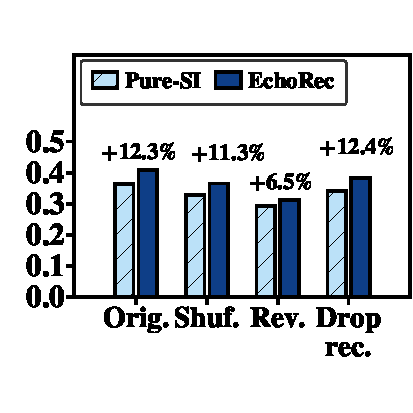
\includegraphics[width=\linewidth,trim=0 22pt 0 0,clip]{sequence_perturb_movies_ndcg10.pdf}
\vspace{-0.60em}
\axissubcaption{(a) Movies}
\end{minipage}\hfill
\begin{minipage}[t]{0.32\textwidth}
\centering
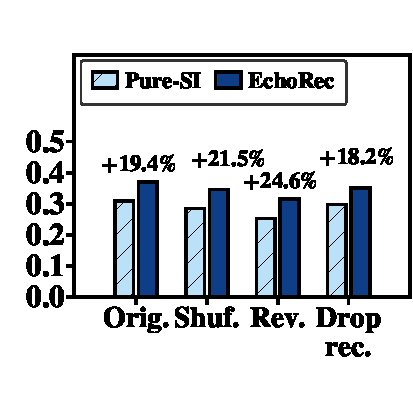
\includegraphics[width=\linewidth,trim=0 22pt 0 0,clip]{sequence_perturb_scientific_ndcg10.pdf}
\vspace{-0.60em}
\axissubcaption{(b) Scientific}
\end{minipage}\hfill
\begin{minipage}[t]{0.32\textwidth}
\centering
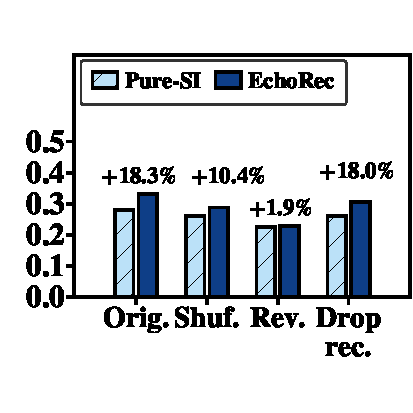
\includegraphics[width=\linewidth,trim=0 22pt 0 0,clip]{sequence_perturb_electronics_ndcg10.pdf}
\vspace{-0.60em}
\axissubcaption{(c) Electronics}
\end{minipage}

\vspace{0.35em}

\begin{minipage}[t]{0.32\textwidth}
\centering
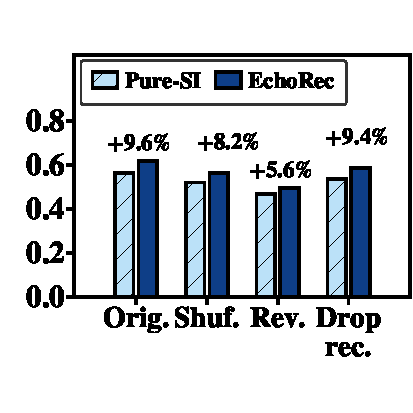
\includegraphics[width=\linewidth,trim=0 22pt 0 0,clip]{sequence_perturb_movies_hr10.pdf}
\vspace{-0.60em}
\axissubcaption{(d) Movies}
\end{minipage}\hfill
\begin{minipage}[t]{0.32\textwidth}
\centering
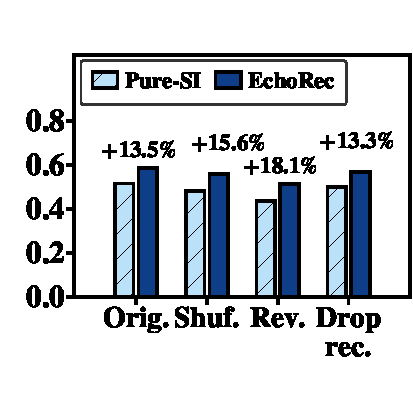
\includegraphics[width=\linewidth,trim=0 22pt 0 0,clip]{sequence_perturb_scientific_hr10.pdf}
\vspace{-0.60em}
\axissubcaption{(e) Scientific}
\end{minipage}\hfill
\begin{minipage}[t]{0.32\textwidth}
\centering
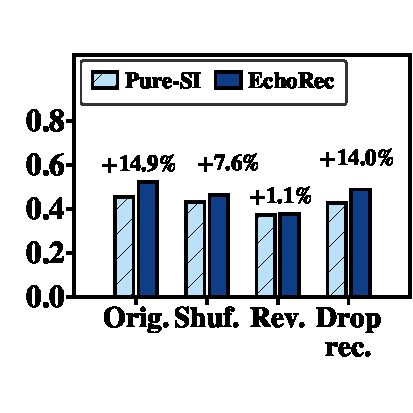
\includegraphics[width=\linewidth,trim=0 22pt 0 0,clip]{sequence_perturb_electronics_hr10.pdf}
\vspace{-0.60em}
\axissubcaption{(f) Electronics}
\end{minipage}
\vspace{-0.20em}
\caption{Sequence perturbation on Movies, Scientific, and Electronics. Top row: NDCG@10; bottom row: HR@10.}
\label{fig:seq_perturb_more_appendix}
\end{figure}
\vspace{-0.65em}

\subsection{Controlled SSHG Diagnosis on Movies, Scientific, and Electronics}
\label{app:rq4_more_datasets}

To complement the CDs example in the main text, we further visualize the controlled SSHG diagnosis on the other three datasets under the same protocol. The same qualitative pattern persists: EchoRec remains above Pure-SI across neighborhood sizes, indicating that teacher-space reshaping consistently improves semantic compatibility before injection and preserves more local sequential structure after injection. These dataset-level plots are consistent with the cross-dataset $k{=}20$ summary in Table~\ref{tab:multidataset_sshg_delta}.

\begin{figure}[!t]
\centering
\begin{minipage}[t]{0.32\textwidth}
\centering
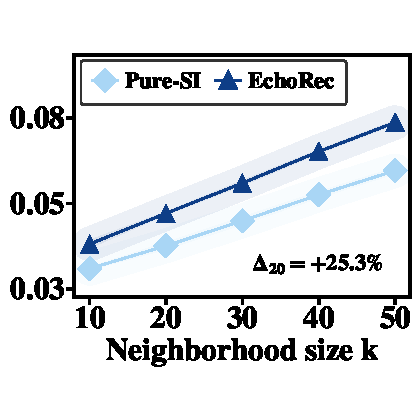
\includegraphics[width=\linewidth,trim=0 22pt 0 0,clip]{movies_sshg_semantic.pdf}
\vspace{-0.60em}
\axissubcaption{(a) Movies}
\end{minipage}\hfill
\begin{minipage}[t]{0.32\textwidth}
\centering
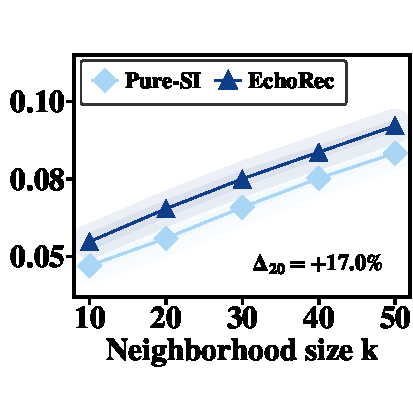
\includegraphics[width=\linewidth,trim=0 22pt 0 0,clip]{scientific_sshg_semantic.pdf}
\vspace{-0.60em}
\axissubcaption{(b) Scientific}
\end{minipage}\hfill
\begin{minipage}[t]{0.32\textwidth}
\centering
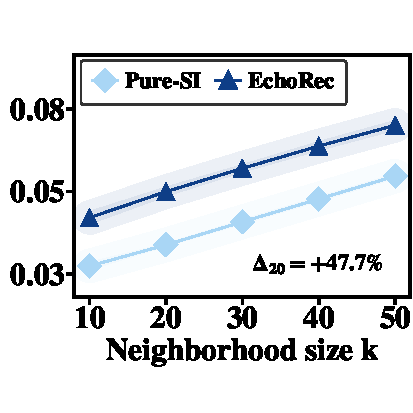
\includegraphics[width=\linewidth,trim=0 22pt 0 0,clip]{electronics_sshg_semantic.pdf}
\vspace{-0.60em}
\axissubcaption{(c) Electronics}
\end{minipage}

\vspace{0.35em}

\begin{minipage}[t]{0.32\textwidth}
\centering

\includegraphics[width=\linewidth,trim=0 22pt 0 0,clip]{movies_sshg_transfer.pdf}
\vspace{-0.60em}
\axissubcaption{(d) Movies}
\end{minipage}\hfill
\begin{minipage}[t]{0.32\textwidth}
\centering
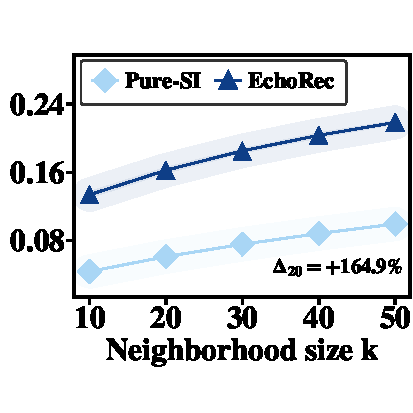
\includegraphics[width=\linewidth,trim=0 22pt 0 0,clip]{scientific_sshg_transfer.pdf}
\vspace{-0.60em}
\axissubcaption{(e) Scientific}
\end{minipage}\hfill
\begin{minipage}[t]{0.32\textwidth}
\centering

\includegraphics[width=\linewidth,trim=0 22pt 0 0,clip]{electronics_sshg_transfer.pdf}
\vspace{-0.60em}
\axissubcaption{(f) Electronics}
\end{minipage}
\vspace{-0.20em}
\caption{Controlled SSHG diagnosis on three additional datasets across neighborhood sizes. Top row: semantic alignment; bottom row: structure transfer.}
\label{fig:rq4_more_datasets_appendix}
\end{figure}

\section{Limitations}
\label{app:limitations}

EchoRec is evaluated under a frozen-LLM retrieval setting with representative teacher backbones and shared benchmarks. The stage-wise design is compatible with different LLM hosts, richer multimodal inputs, and alternative serving pipelines. EchoRec uses offline semantic-asset construction and two-stage training, shifting additional computation to reusable preprocessing and training stages while keeping online inference lightweight.

\section{Broader Impacts and Assets}
\label{app:broader_assets}

EchoRec may improve LLM-based sequential recommendation by making transferred sequential cues more reliable. Potential negative impacts include amplifying historical popularity bias, exposing user-preference patterns if interaction logs are mishandled, and increasing computation compared with lightweight recommenders. Our experiments use public benchmark datasets and cited baseline/model assets; the released code will document reproduction details and asset terms.

\section{Future Work}
\label{app:future_work}

Future work can study more efficient semantic-asset construction, parameter-efficient adaptation, and evaluation with a wider range of LLM hosts and teacher backbones. Another promising direction is extending the current setting to richer multimodal or online recommendation scenarios, so that large-small collaboration remains effective and practical in real-world pipelines.

\clearpage
\input{checklist}

\end{document}



